%%%%%%%%%%%%%%%%%%%%%%%%%%%%%%%%%%%%%%%%
% This template has been downloaded from https:overleaf.com/
% Licence: CC-BY
%%%%%%%%%%%%%%%%%%%%%%%%%%%%%%%%%%%%%%%%
\documentclass[12pt, letterpaper, oneside]{report}
\usepackage[lmargin=1in, rmargin=0.5in, tmargin=0.55in, bmargin=0.5in]{geometry}

%\usepackage[cp1251]{inputenc}
%\usepackage[russian, english]{babel}


\usepackage[utf8x]{inputenc} 

\usepackage[T2A]{fontenc} 

\usepackage[english,russian]{babel} 


\usepackage{euscript}	 % Шрифт Евклид
\usepackage{mathrsfs} % Красивый матшрифт
\usepackage{amssymb,amsfonts,amsmath,mathtext}
\usepackage{cmap} % чтобы работал поиск по PDF
%\usepackage[pdftex]{graphicx}
%\pdfcompresslevel=9 % сжимать PDF
%\else
%\usepackage{graphicx}

% \usepackage[utf8]{inputenc}
%\usepackage{lipsum}
\usepackage{gensymb}
\usepackage{fancyhdr}


\usepackage{graphicx}   % Written by David Carlisle and Sebastian Rahtz
\usepackage{subcaption}
\usepackage{url}        % Written by Donald Arseneau
 

\usepackage{float}

\usepackage[toc,page]{appendix}
\pagestyle{fancy}
%\fancyhead[]

%%%%%%%%%%%%%%%%%%%%%%%%%%%%%%%%
%% Copyright (C) 2018 Almas Askarbekov.
%% License: CC-BY.
%%%%%%%%%%%%%%%%%%%%%%%%%%%%%%%%
\begin{document}
\selectlanguage{english}
\fancyhead[L]{\slshape \MakeUppercase Diamond section}
\fancyhead[R]{Almas Askarbekov}
\begin{titlepage}

\newcommand{\HRule}{\rule{\linewidth}{0.5mm}} % Defines a new command for the horizontal lines, change thickness here

\center % Center everything on the page
 
%----------------------------------------------------------------------------------------
%   HEADING SECTIONS
%----------------------------------------------------------------------------------------


%\textsc{\large Same problem, different angle}\\[0.5cm] 

%----------------------------------------------------------------------------------------
%   TITLE SECTION
%----------------------------------------------------------------------------------------

\HRule \\[0.8cm]
{ \huge \bfseries Doubling the cube}\\[0.4cm] % Title
\HRule \\[1.5cm]
\textsc{\large  Same problem, different angle.}\\[0.5cm] 
%----------------------------------------------------------------------------------------
%   AUTHOR SECTION
%----------------------------------------------------------------------------------------

\begin{minipage}{0.8\textwidth}
\begin{center} \large


\end{center}

\begin{center}

\end{center}

\end{minipage}


\begin{figure}[h]
\centerline{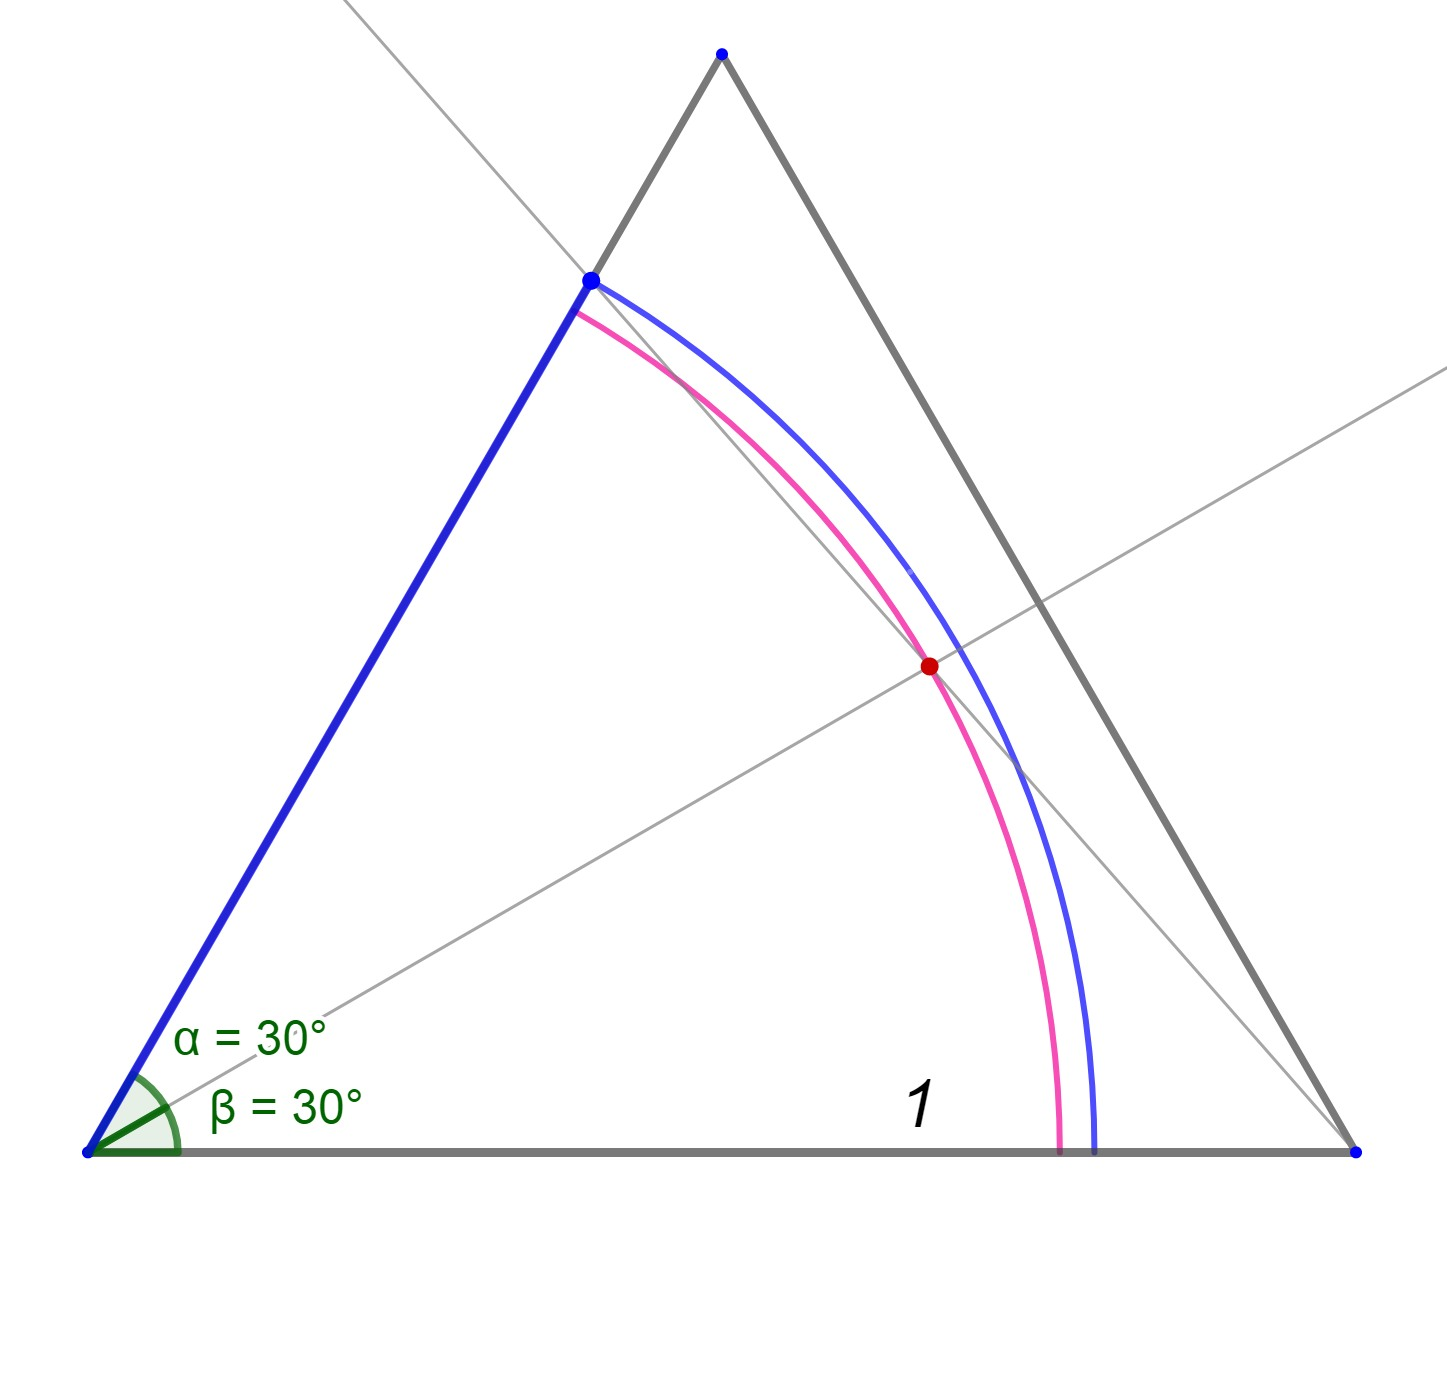
\includegraphics[scale=0.2]{images/ds_tr.jpg}}

\label{logo}
\end{figure}
\textsc{\LARGE Almas Askarbekov }\\[1.5cm]
\begin{center}
	\large {jobspace@yandex.com}\\	
\end{center}
\end{titlepage}


\begin{center}
\section*{Abstract}
\end{center}
Doubling the cube also known as the Delian problem is one of the three famous geometric problems of antiquity, unsolvable by compass and straightedge construction. Given the edge of a cube, the problem requires the construction of the edge of a second cube, whose volume is double that of the first.
\\
The only tools allowed for the construction is the unmarked straightedge and compass.
\\
In algebraic terms, doubling a unit cube requires the construction of a line segment of length x, where $x^{3} = 2$; in other words $x =\sqrt[3]{2}$.\\
Pierre Wantzel proved in 1837 that the $\sqrt[3]{2}$ can not be constructed using a compass and straightedge.
\\
\begin{figure}[h]
	\centering
	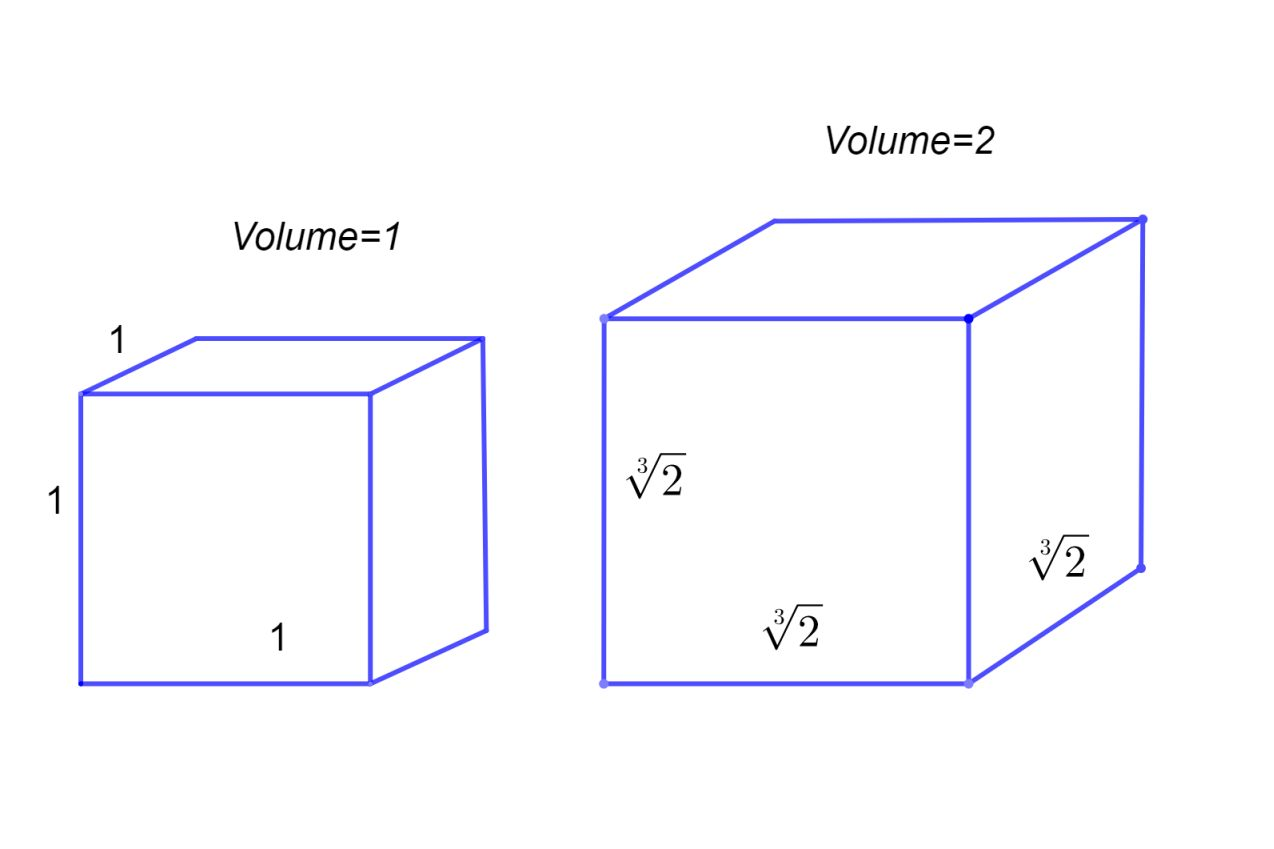
\includegraphics[width=0.7\linewidth]{images/cubes.jpg}
	\label{fig:cubes}
\end{figure}
\begin{figure}[h]
	\centering
	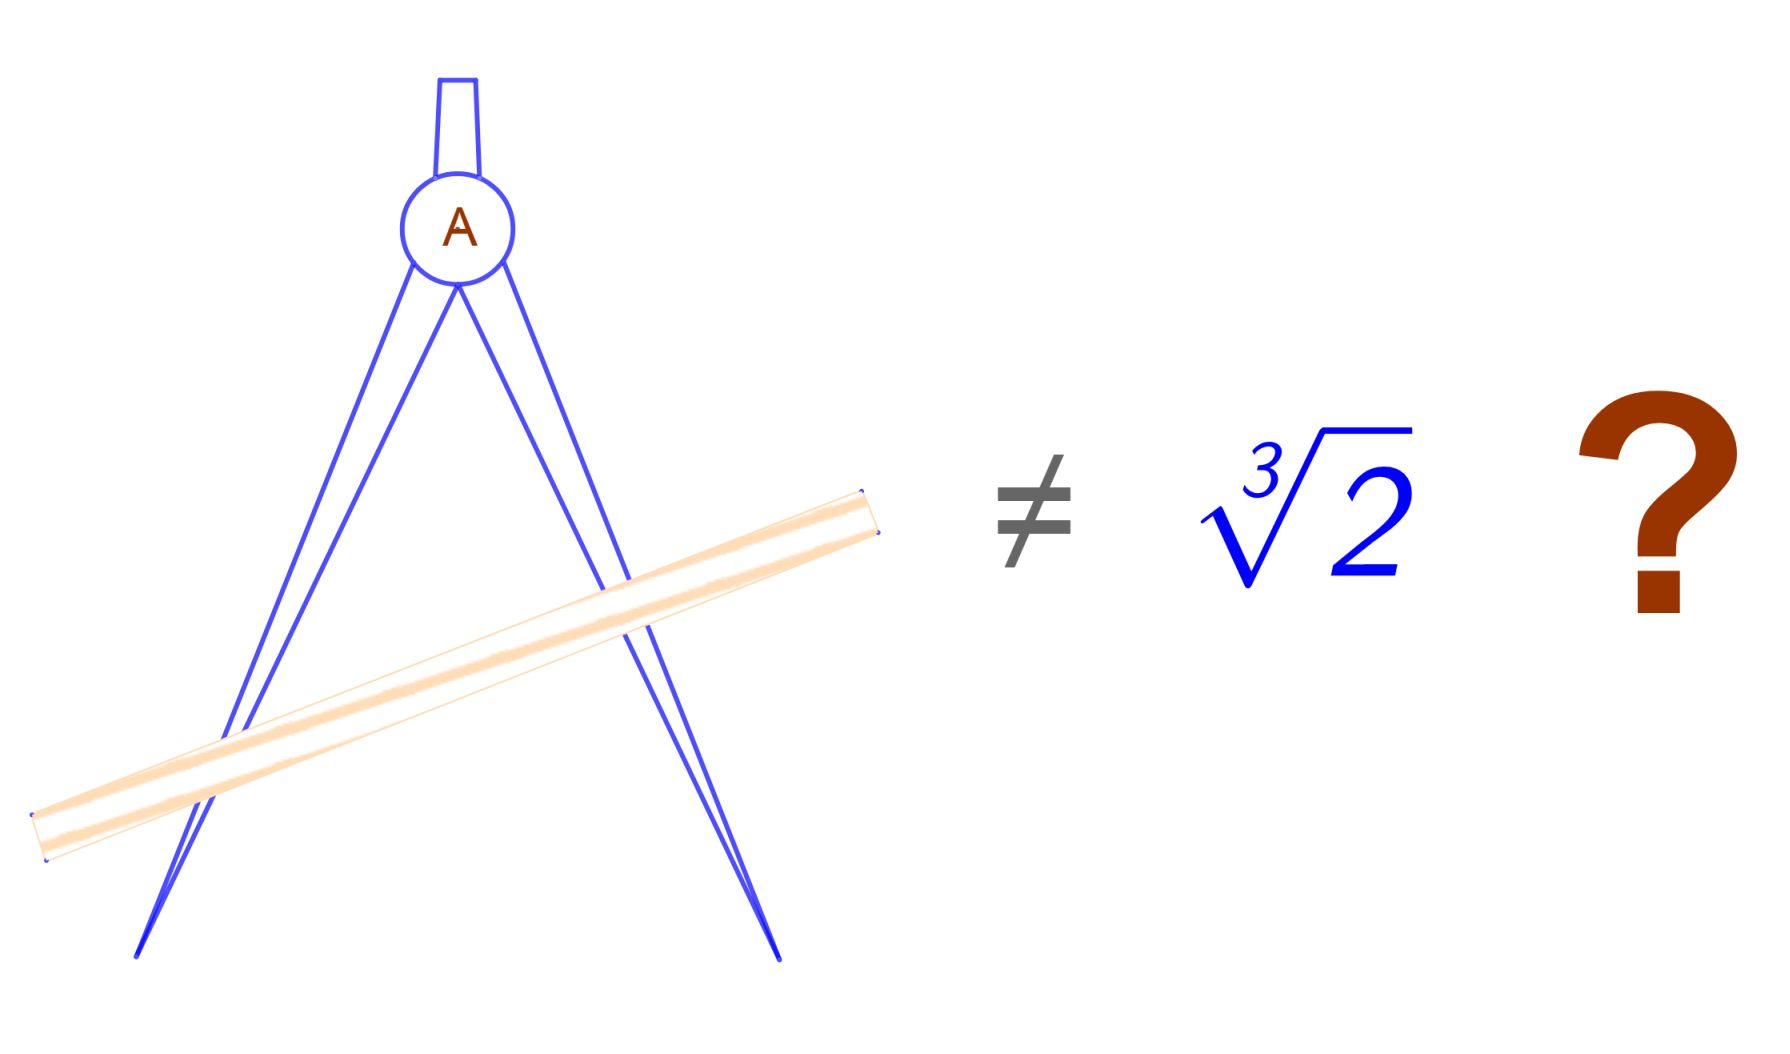
\includegraphics[width=0.8\linewidth]{images/compass.jpg}
	\label{fig:compass}
\end{figure}
\newpage

\tableofcontents

\chapter{}

\section{Construction}
\begin{enumerate}
	\item Let's construct base lines and circles with radius $r=1$ as shown in fig. 1.1.
\begin{figure}[H]
	\centerline{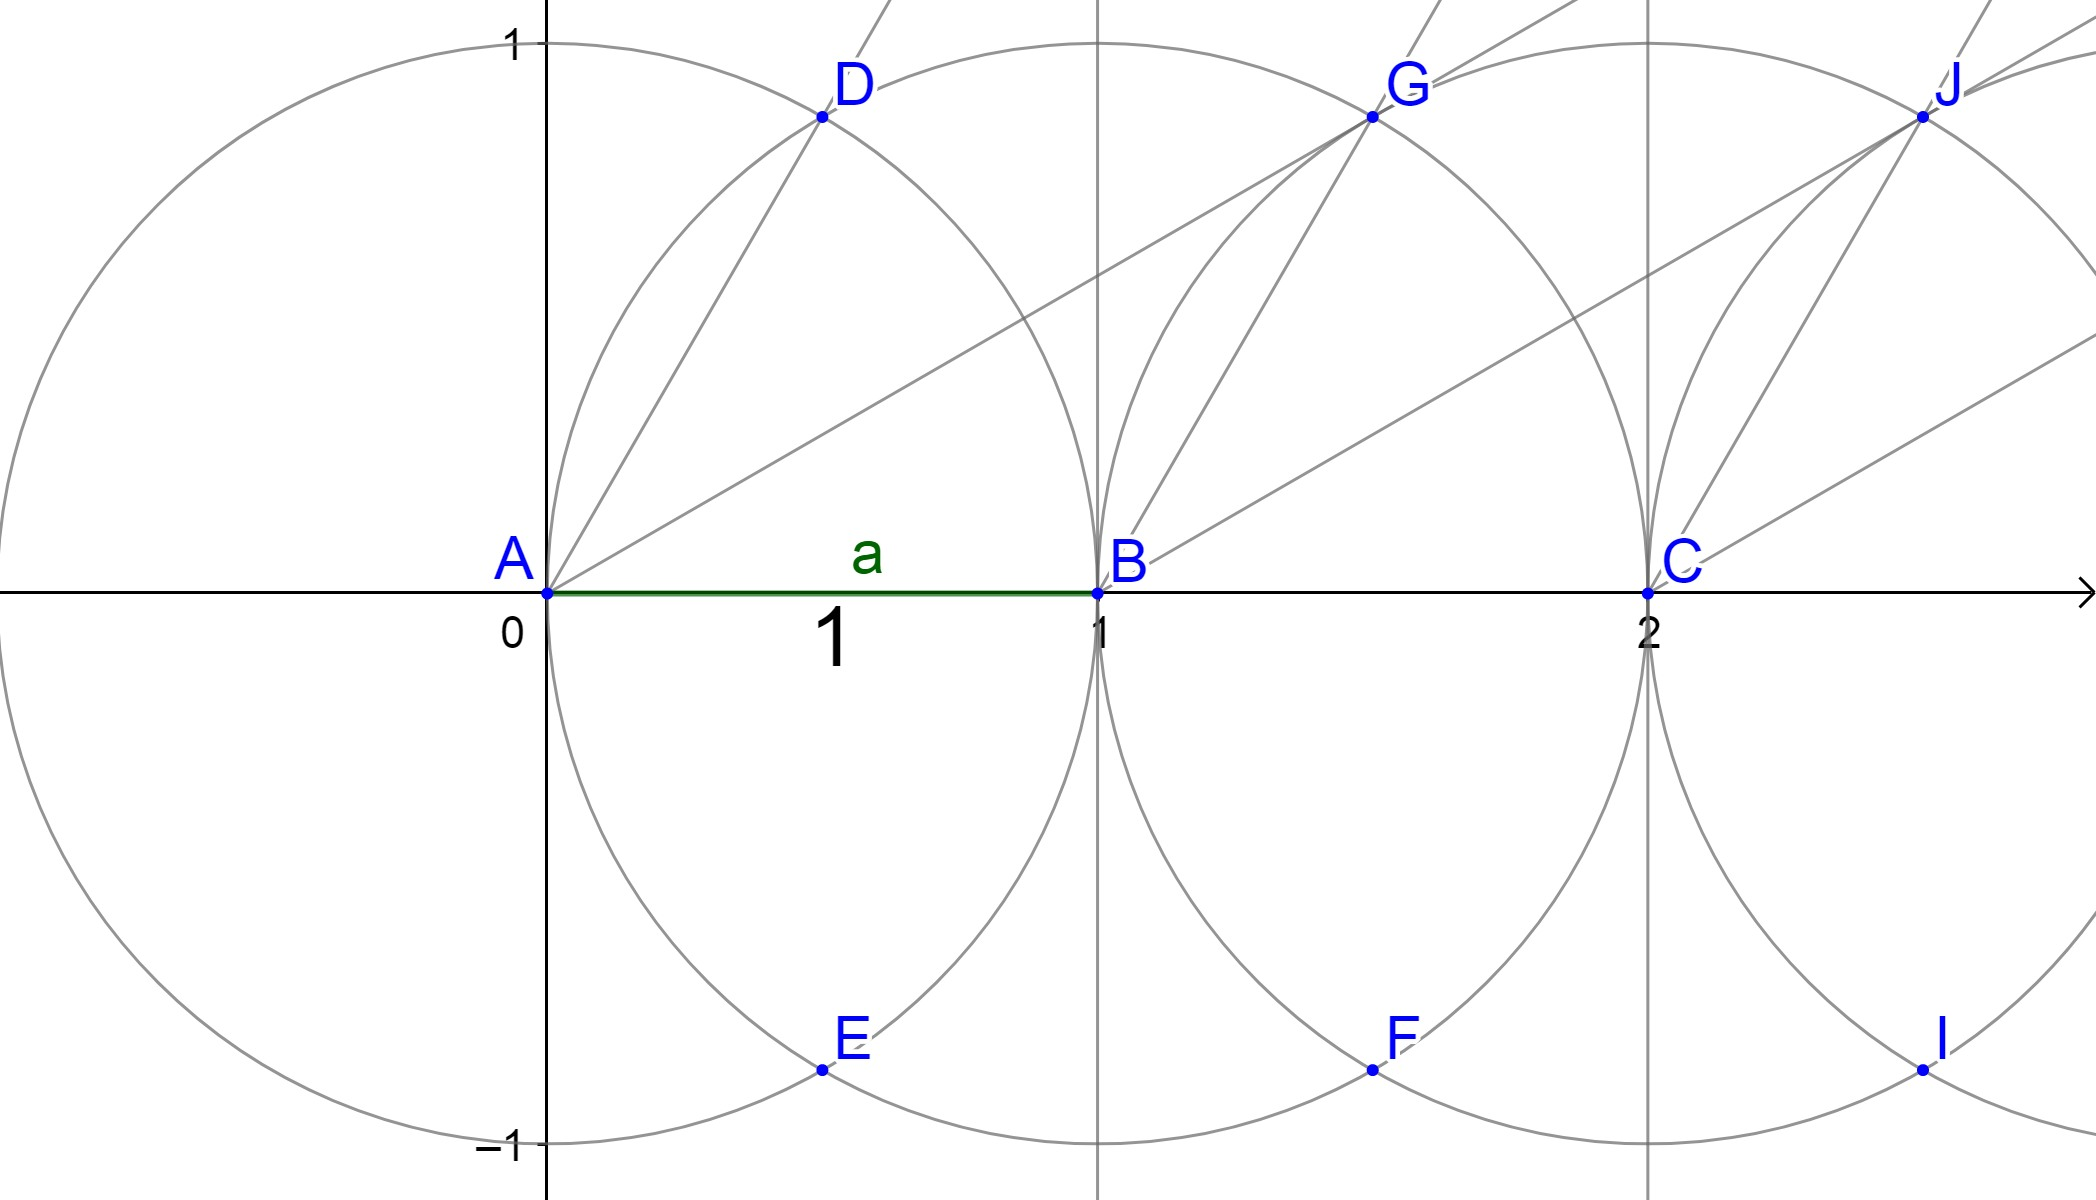
\includegraphics[scale=0.18]{img/basic.jpg}}
	\caption{Basic circle structure}
	\label{fig:basic}
\end{figure}
	
	\item Then let's construct a right triangle $\triangle ANB$ (see fig. \ref{fig:1_anb}) whith an arbitrary short leg $t=0.75$ \\
\begin{figure}[H]
	\centerline{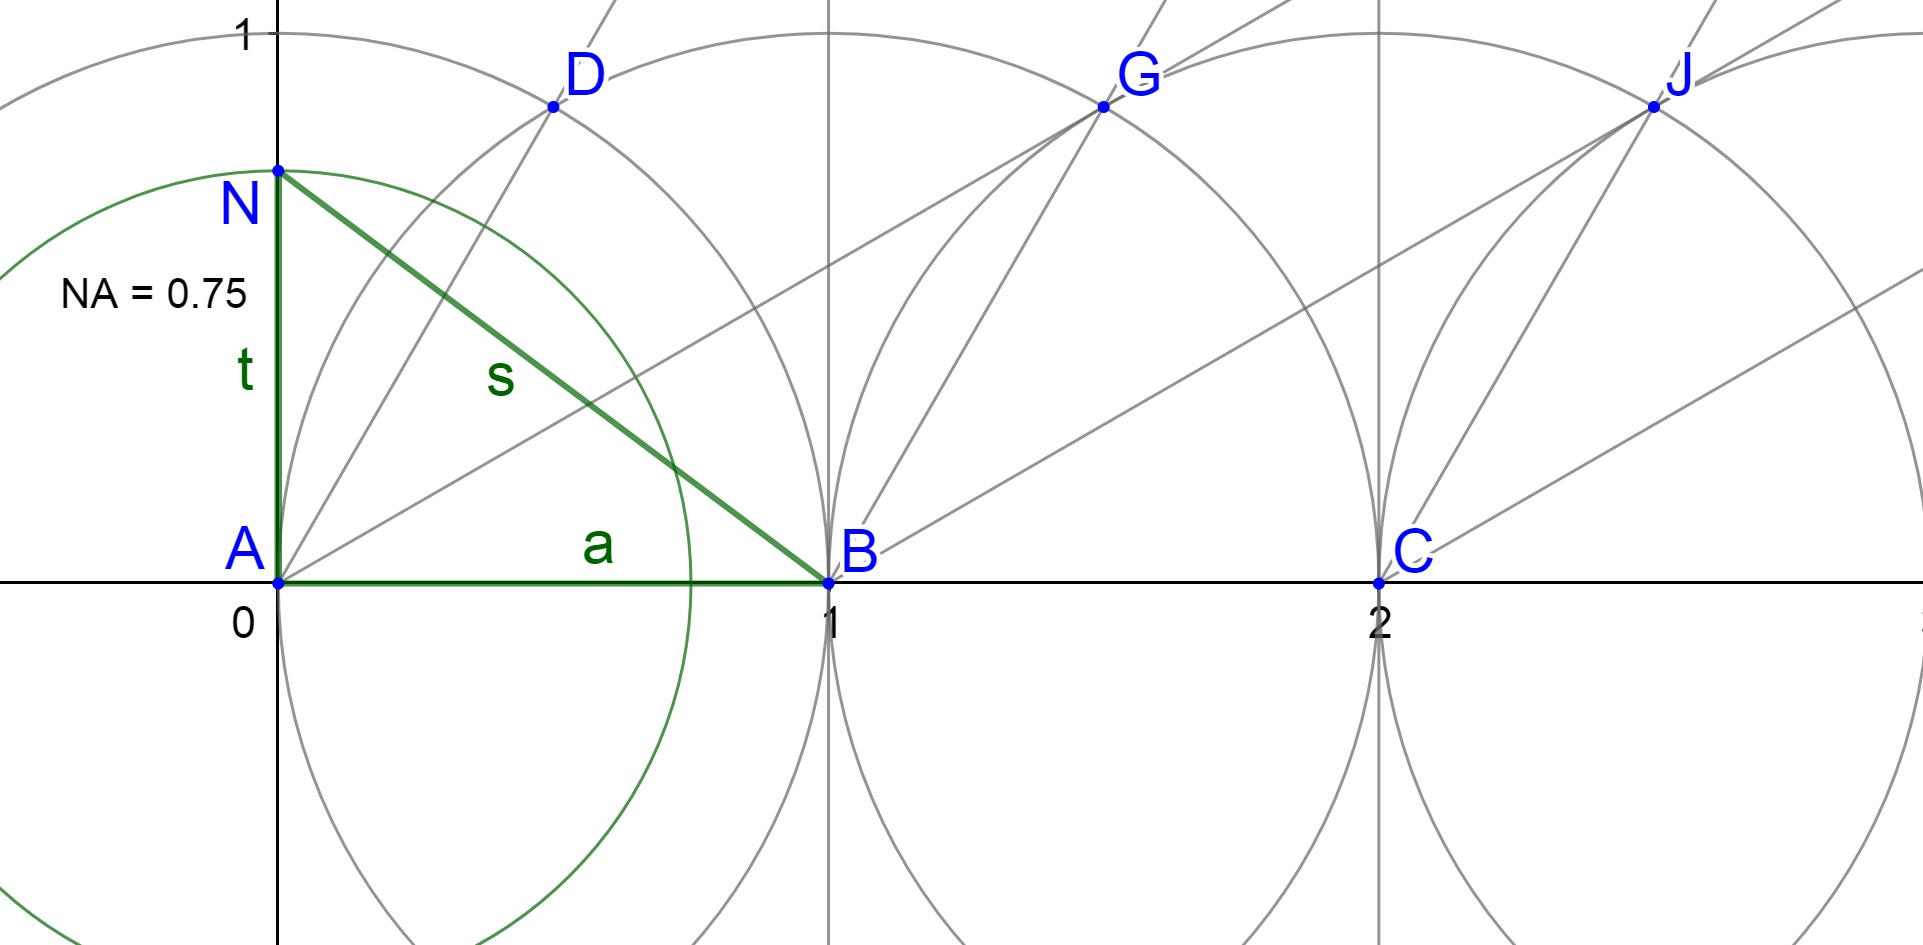
\includegraphics[scale=0.18]{img/1_anb.jpg}}
	\caption{Right triangle}
	\label{fig:1_anb}
\end{figure}	
	Then we calculate the hypotenuse using the Pythagorean theorem:
\begin{equation}
s=\overline{NB}=\sqrt{a^{2}+t^{2}}=\sqrt{1^{2}+0.75^{2}}=1.25
\end{equation}
\\
	\item Hence the ratio of the leg to the hypotenuse:
\begin{equation}
	\dfrac{a}{s}=\cos \angle ABN=\dfrac{1}{1.25}=0.8
\end{equation}
\\
To build this relation, let's draw a line through the points $N$ and $B$. We will get the point $O$ and the point $P$. (see fig. \ref{fig:2_second})
\begin{figure}[h]
	\centerline{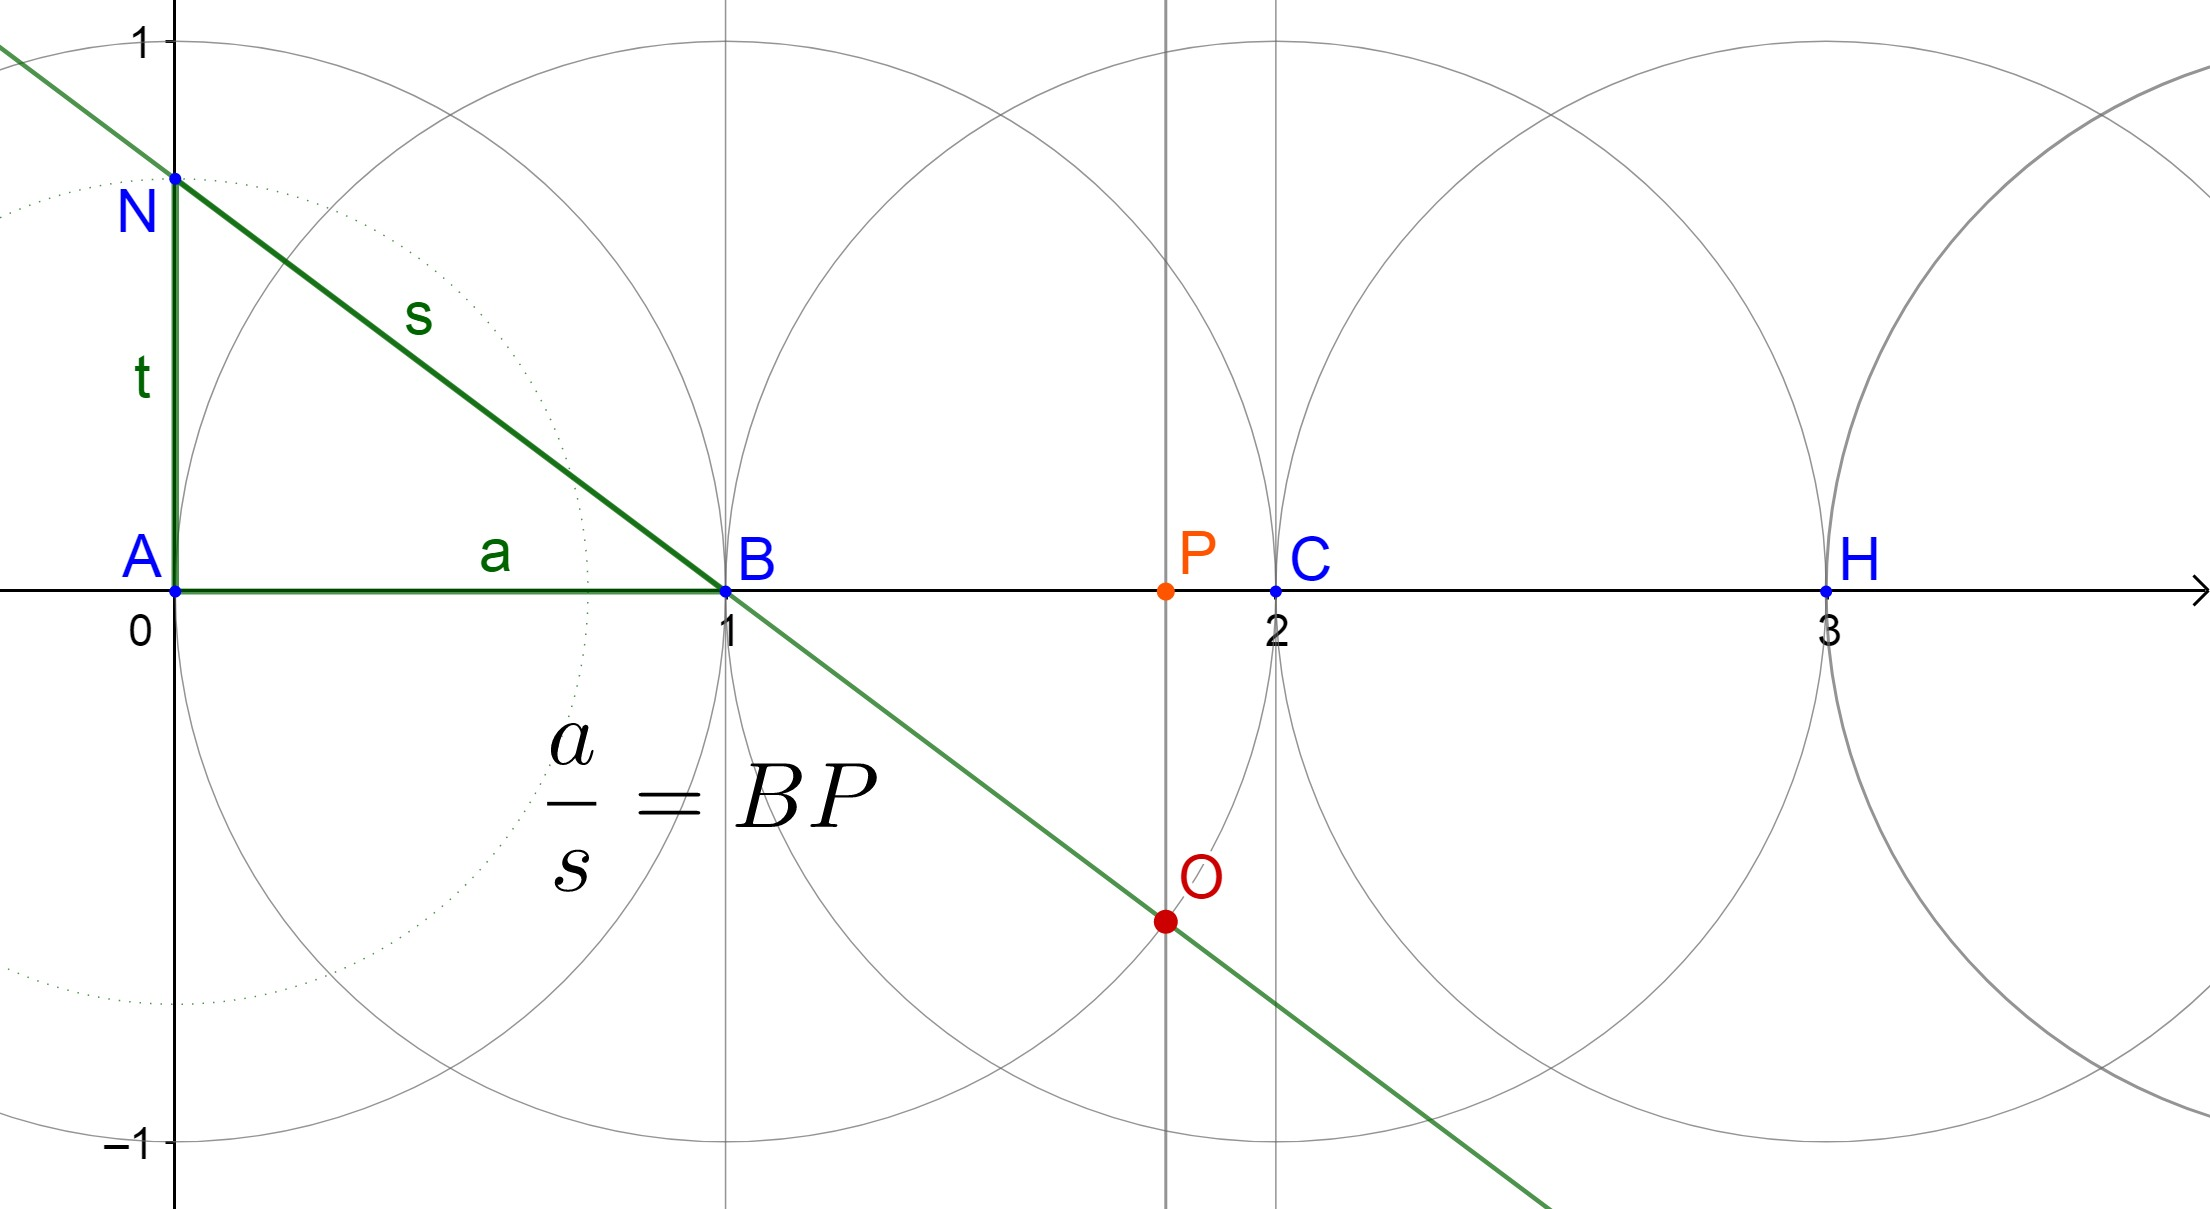
\includegraphics[scale=0.2]{img/anbo.jpg}}
	\caption{}
	\label{fig:2_second}
\end{figure}
\vfill
	\item Now let's construct a circle with center $B$ and radius = $BP$ = $0.8$ (see fig. \ref{fig:anbop})\\ 
\begin{figure}[h]
	\centerline{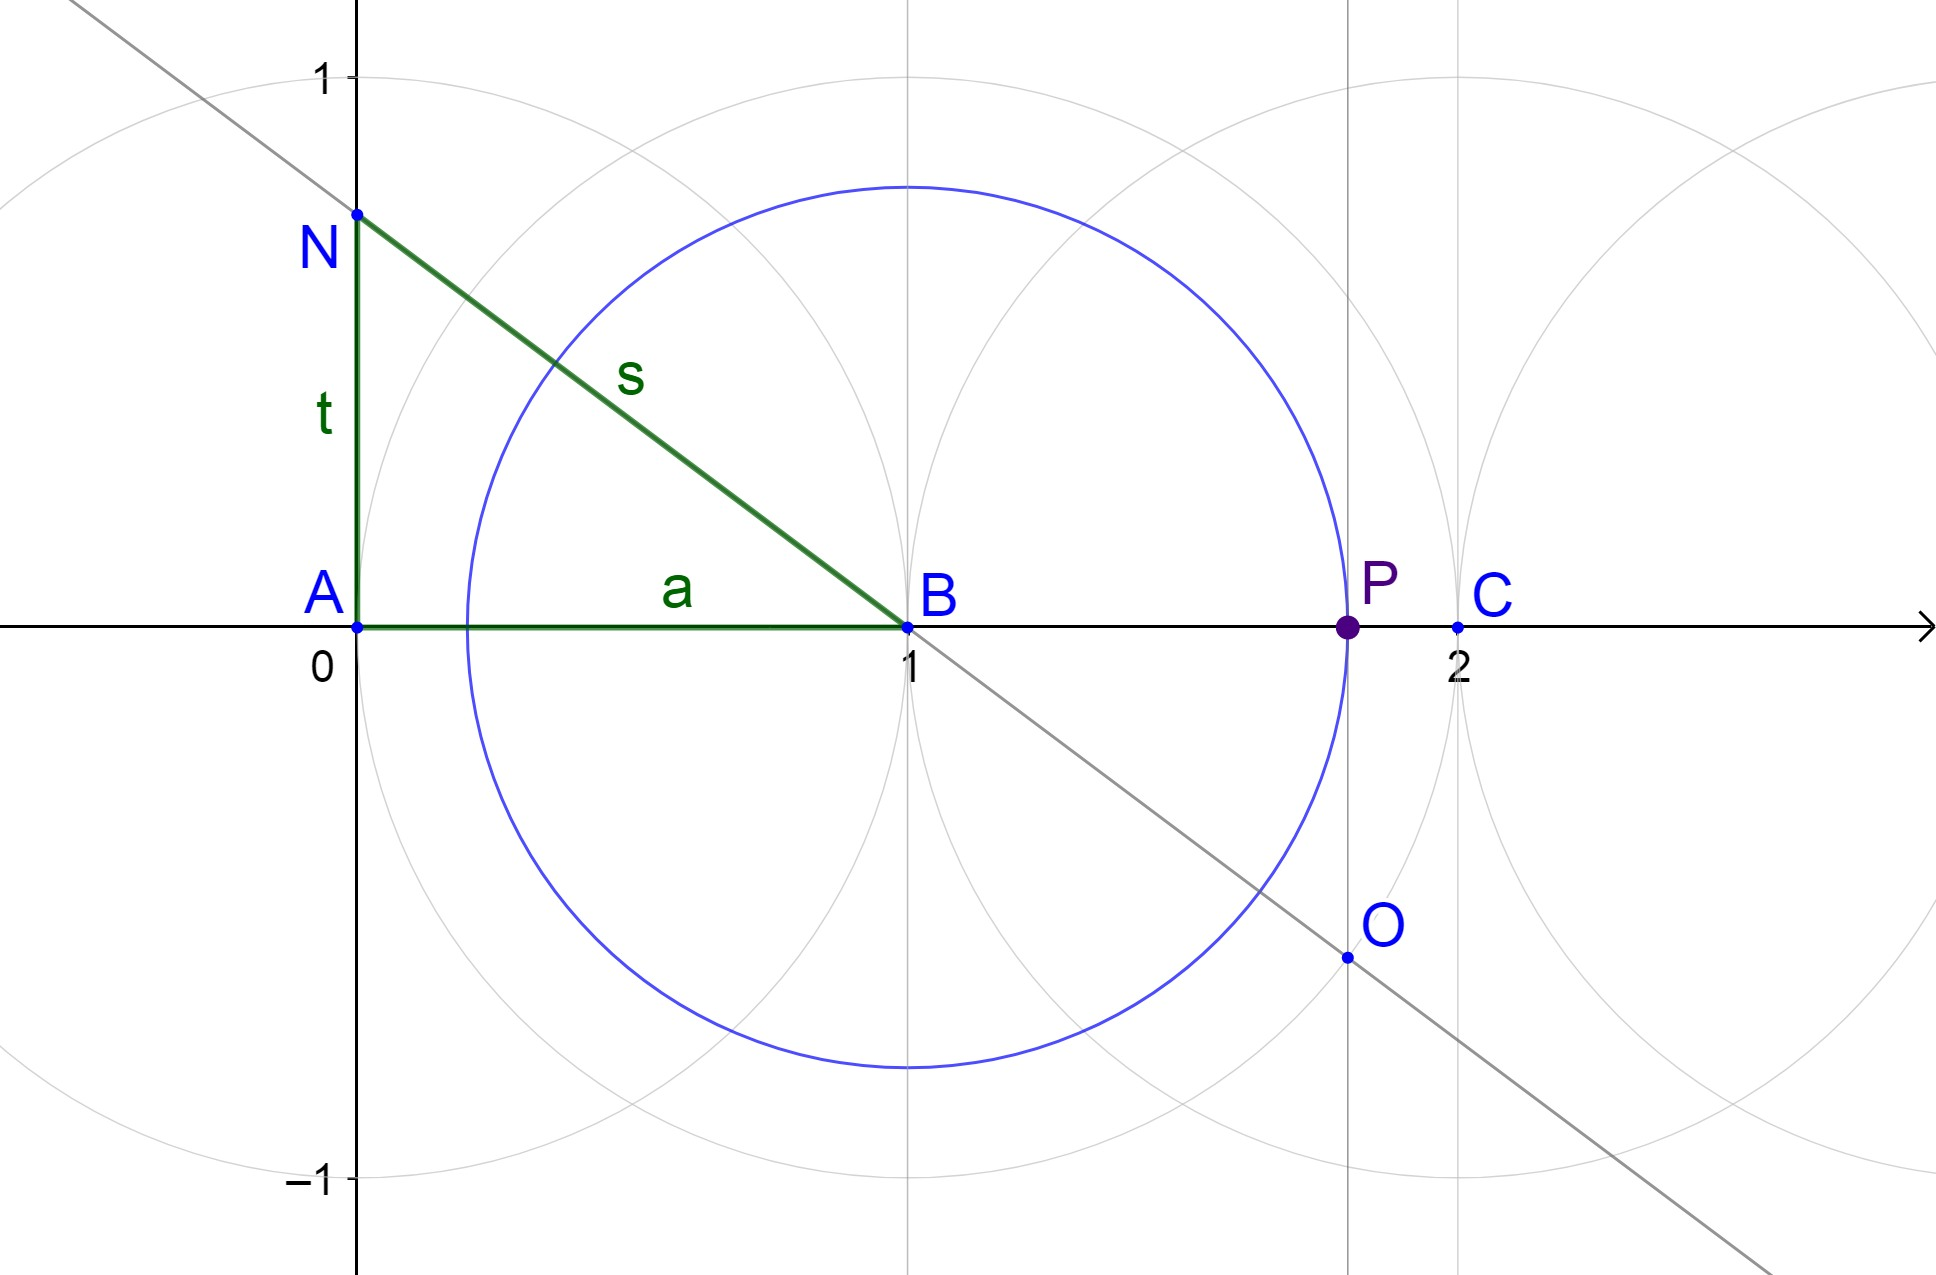
\includegraphics[scale=0.15]{img/anbop.jpg}}
	\caption{}
	\label{fig:anbop}
\end{figure}
\newpage
	\item Then we construct a ray from the point $C(2,0)$ through the point $Q$ which is the intersection of the circle with center $B$ and the segment $\overline{BG}$. (see fig. \ref{fig:anbopq}).
\begin{figure}[h]
	\centerline{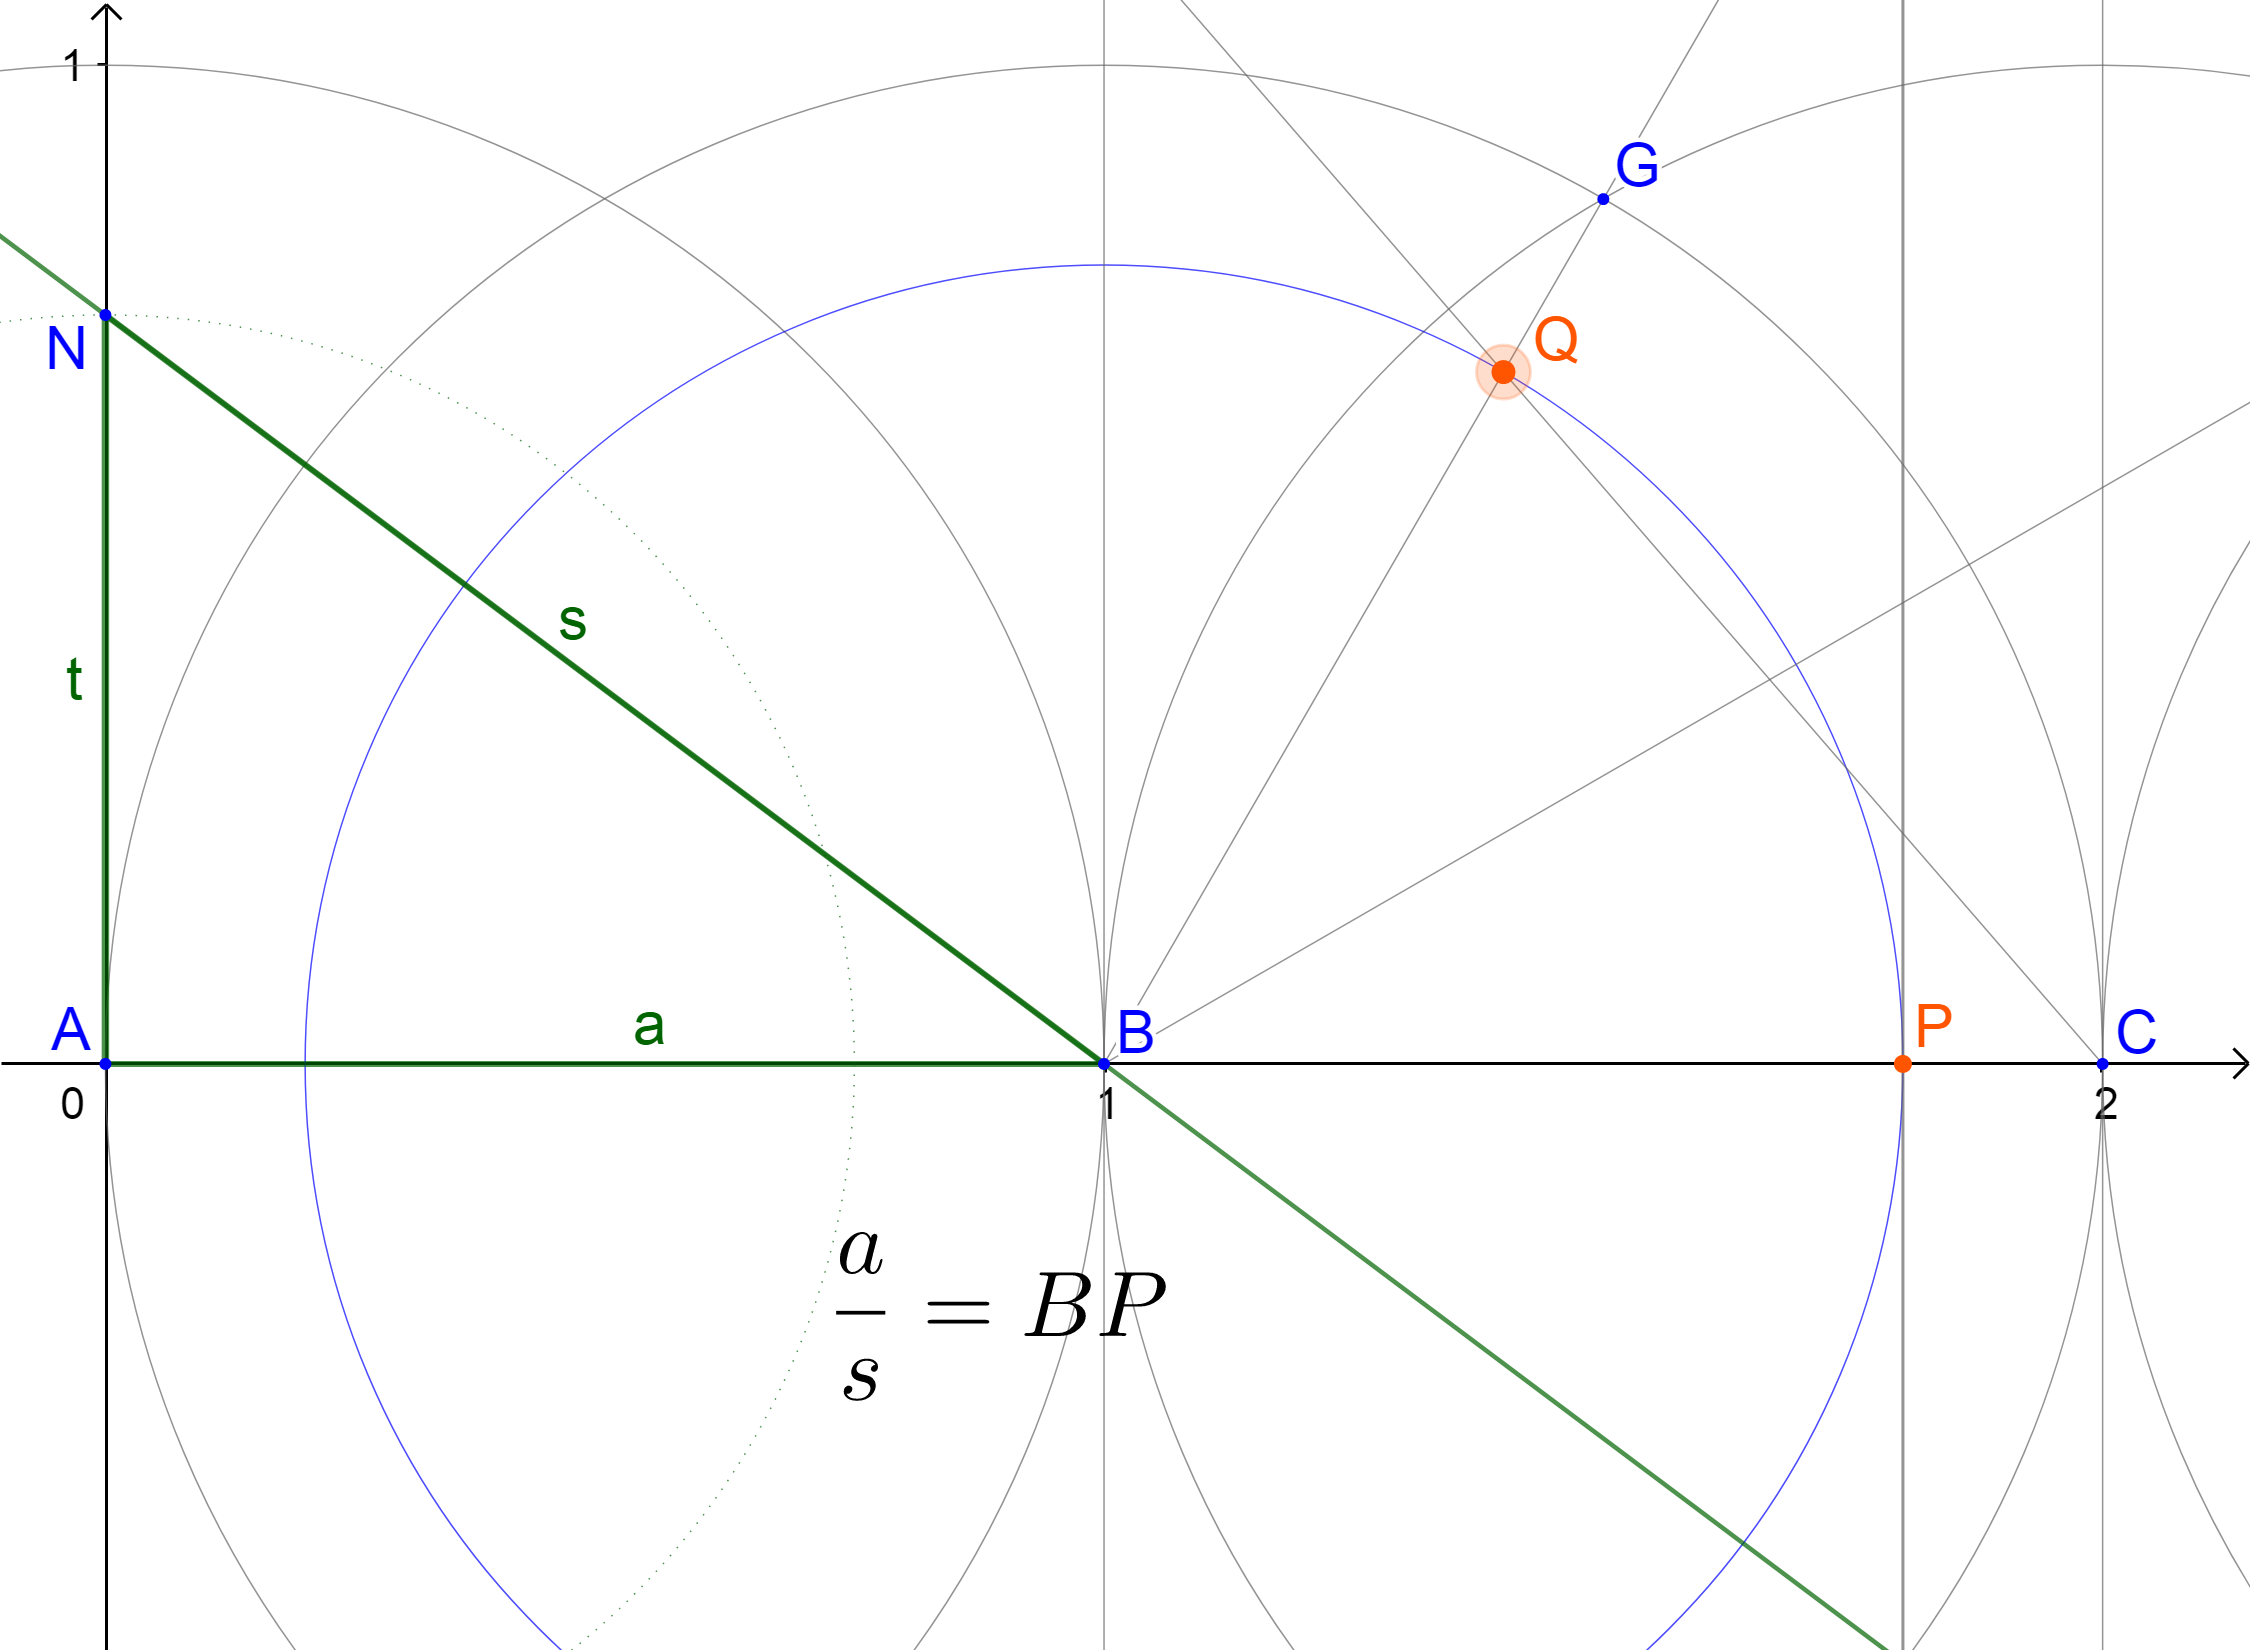
\includegraphics[scale=0.15]{img/anbopQ.png}}
	\caption{}
	\label{fig:anbopq}
\end{figure}
	\item Then we get the point $R$ as shown in fig. \ref{fig:anbopqr}\\
\begin{figure}[h]
	\centerline{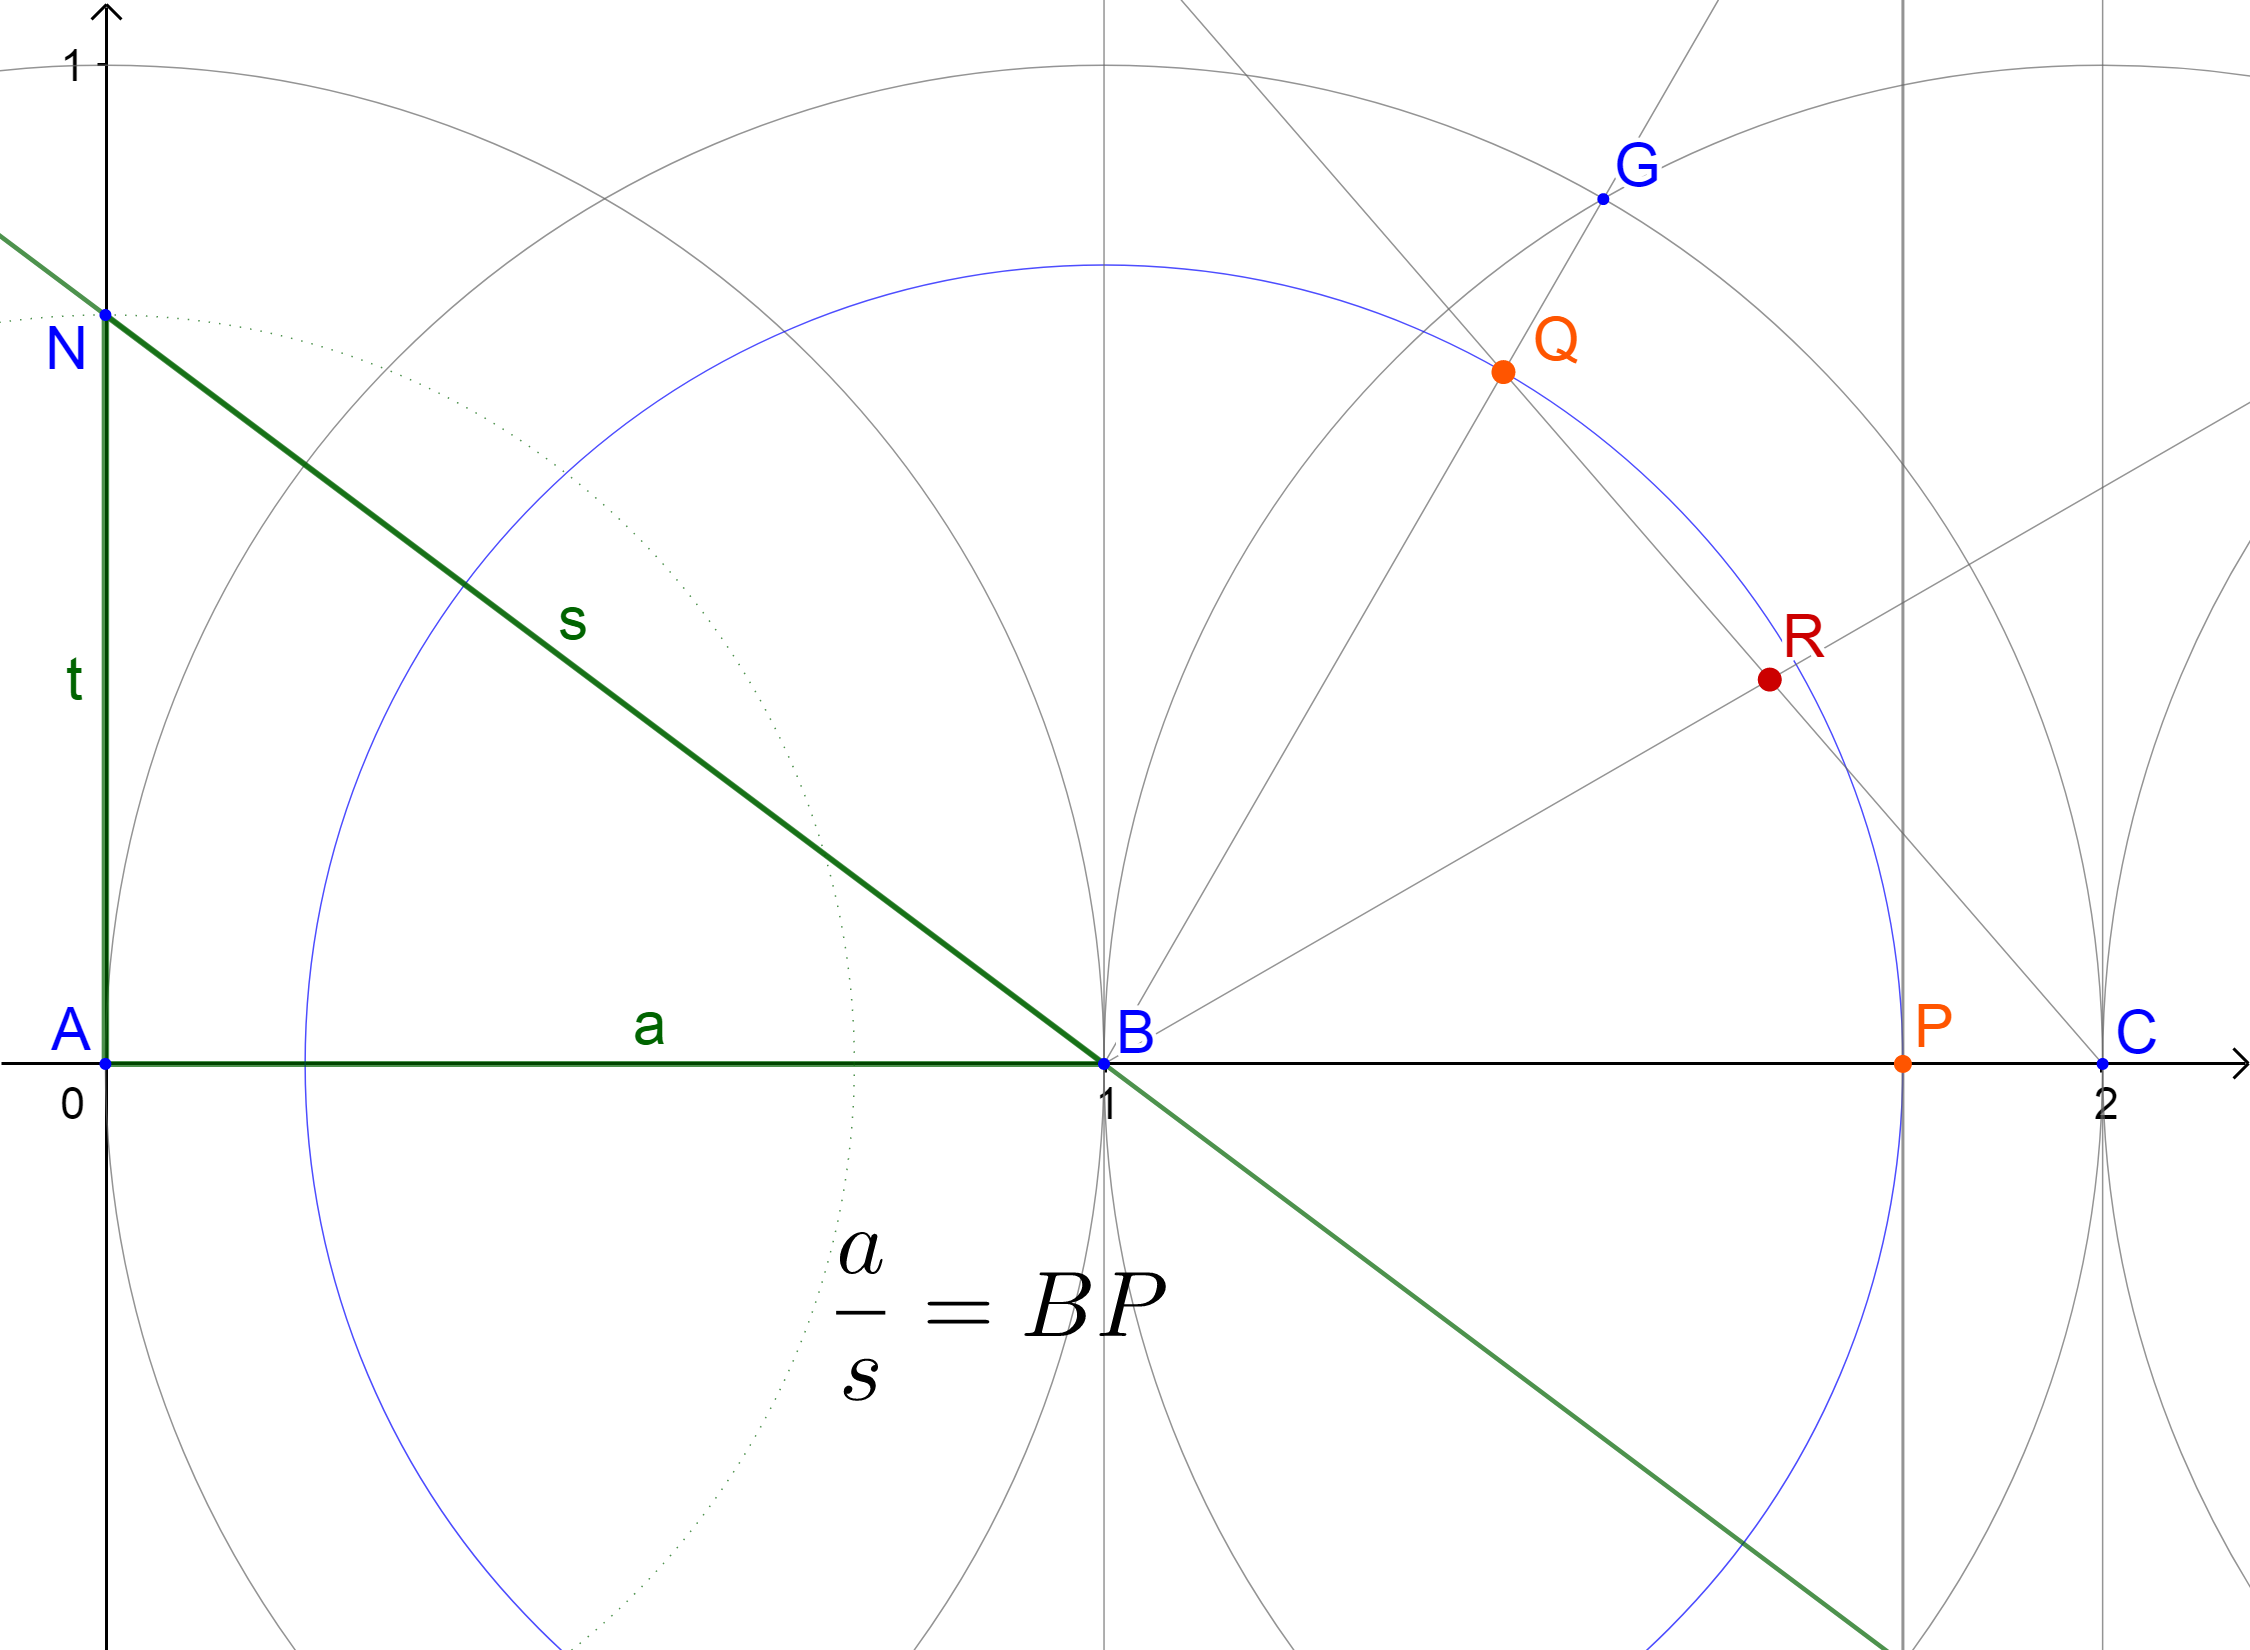
\includegraphics[scale=0.14]{img/anbopqR.png}}
	\caption{}
	\label{fig:anbopqr}
\end{figure}\\
	Segment $BR$ is a bisector of a $\triangle$ $BQC$  (see fig. \ref{fig:bqc})
\newpage
Now we have a $\triangle$ $BQC$ where $BQ=BP=\dfrac{a}{s}=\cos \angle ABN$.
\begin{figure}[H]
		\centerline{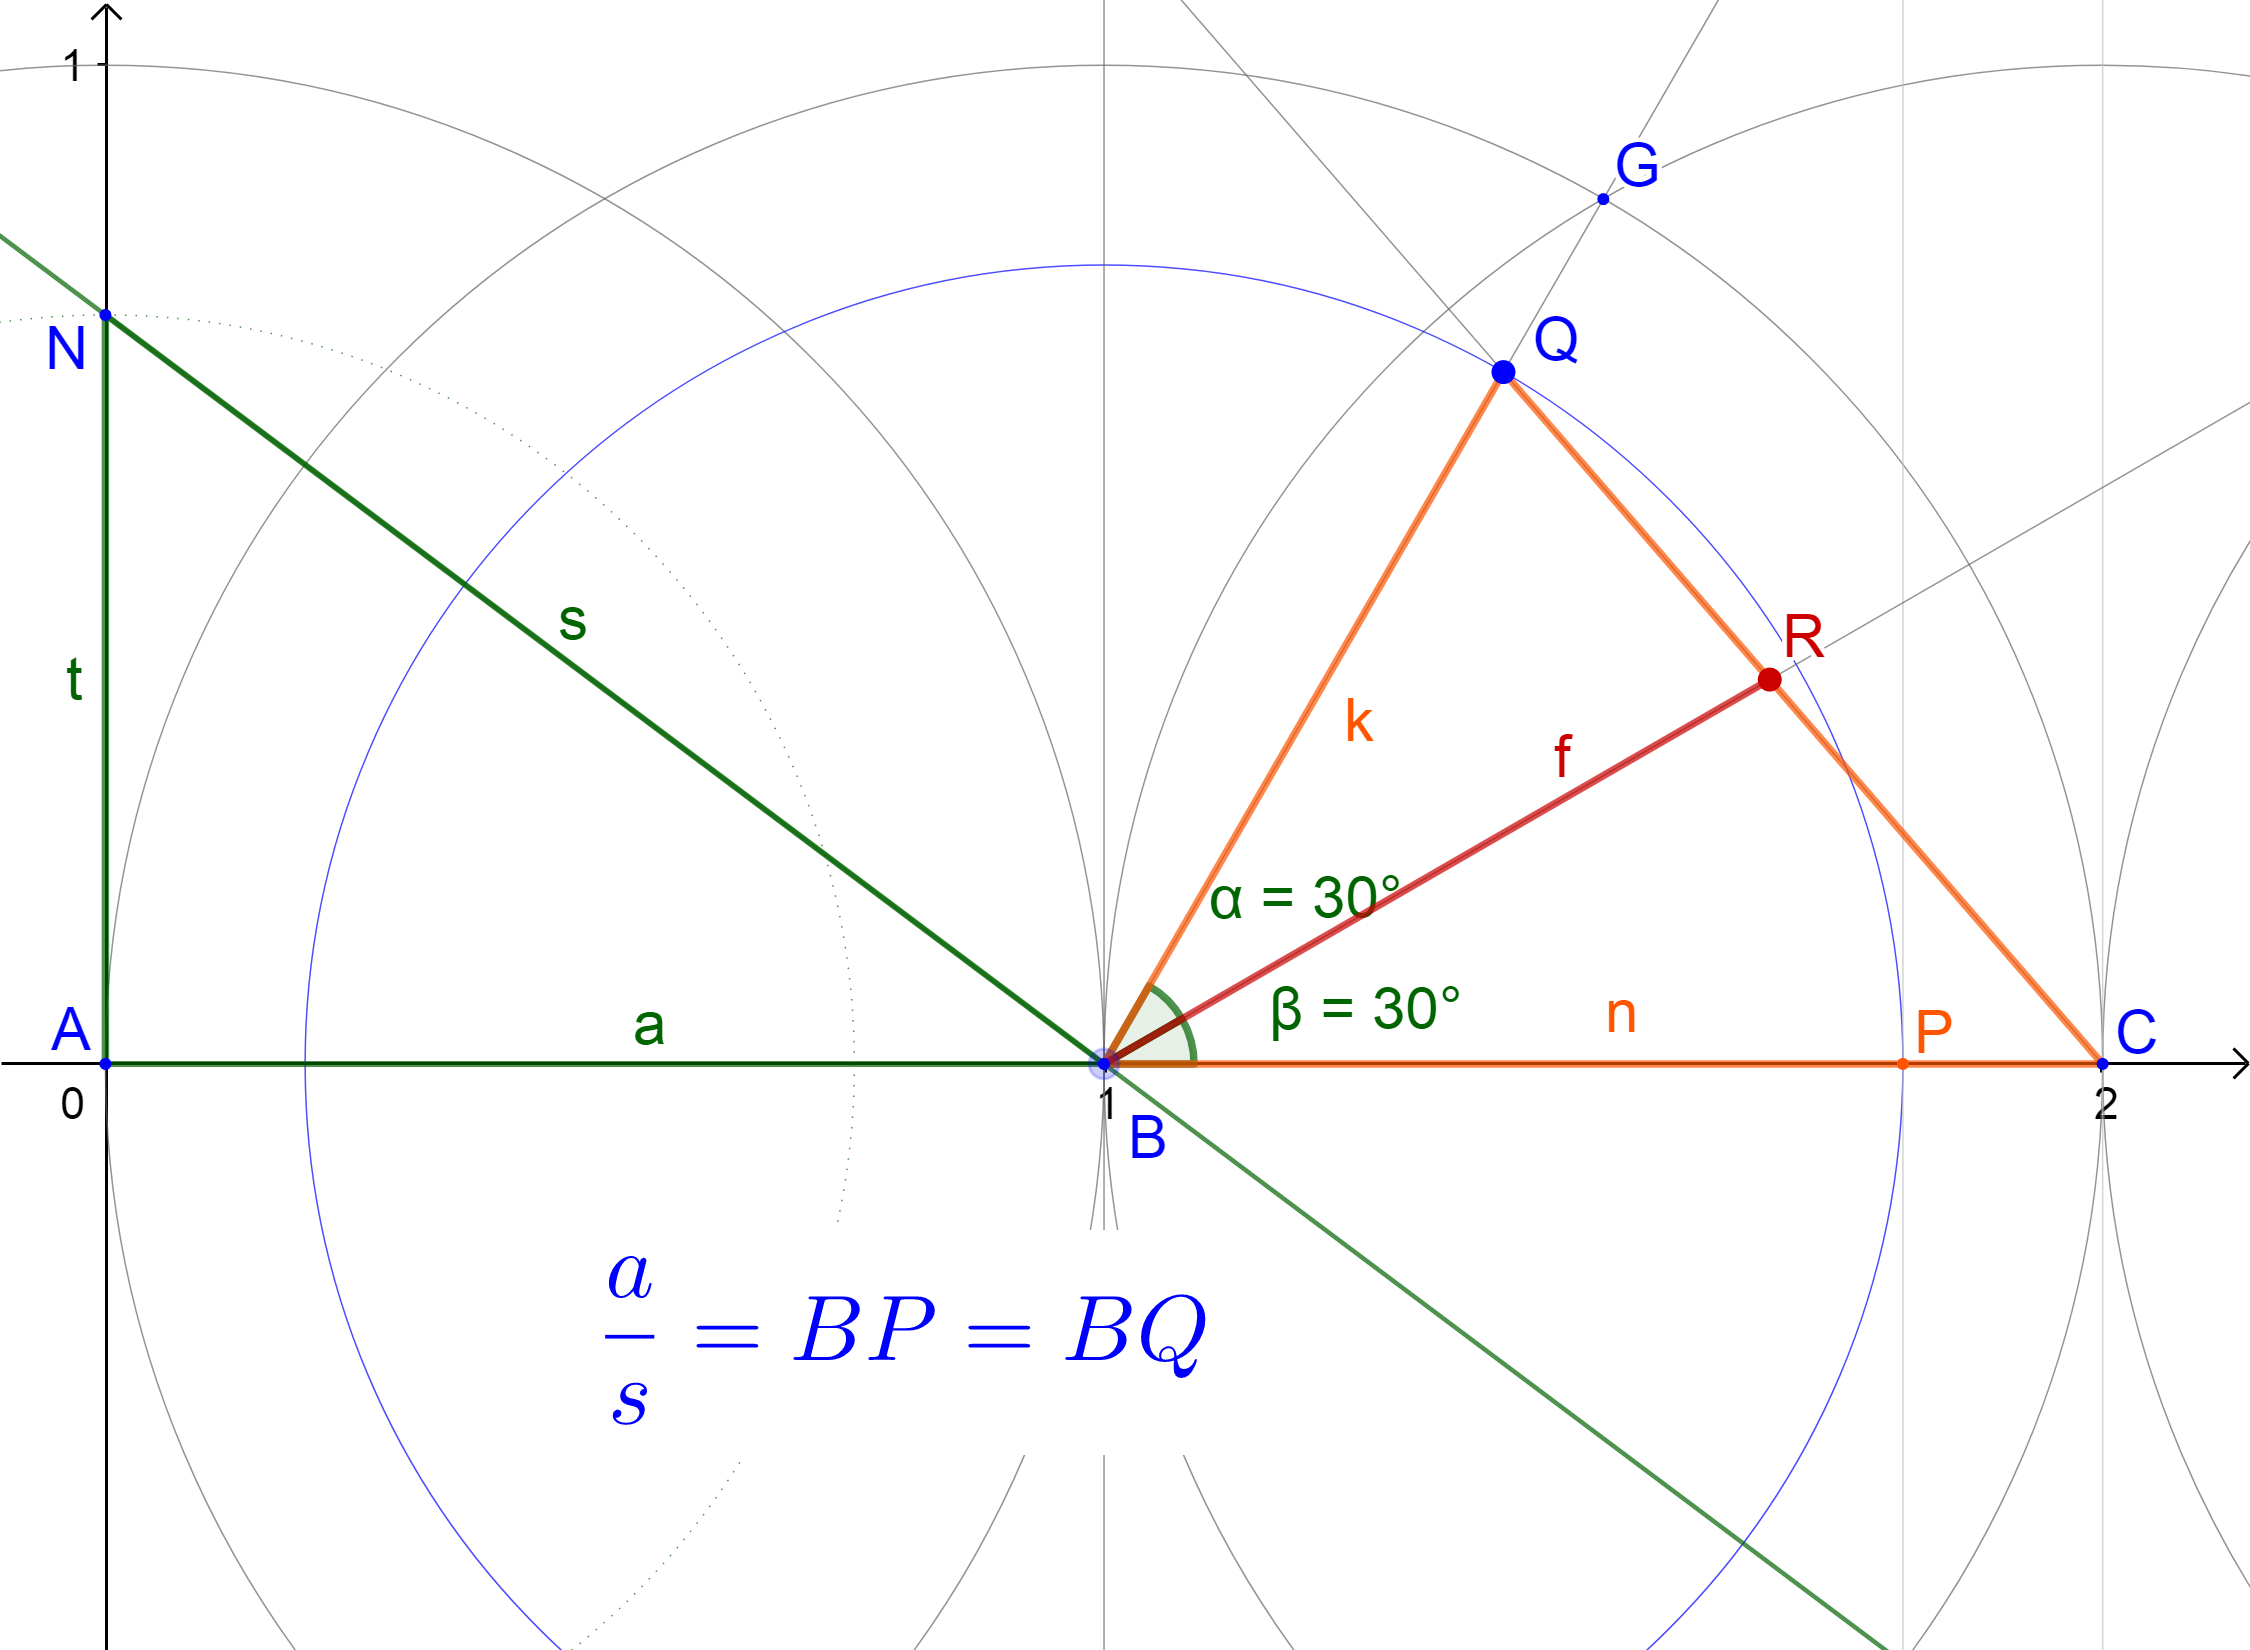
\includegraphics[scale=0.15]{img/BQC.png}}
		\caption{Triangle $BQC$}
		\label{fig:bqc}
\end{figure}
	\item Let's calculate the bisector $BR$ using the formula for the length of the bisector for an angle of 60 degrees:	
\begin{equation}
f=\frac{2nk}{k+n}\times \cos 60\degree = \frac{2nk}{k+n}\times\frac{\sqrt{3}}{2}
\end{equation}\\
	where:  $k=BQ=0.8$; $n=BC=1$; hence:
\begin{equation}	
f=\frac{2\times0.8}{1+0.8}\times\frac{\sqrt{3}}{2}\approx 0.769800358919501
\end{equation}
	\item Let's construct a circle with radius = $f$ and center at the point $B(1,0)$ and get the point $D$ (see Fig. \ref{circle})
\begin{figure}[h]
	\centerline{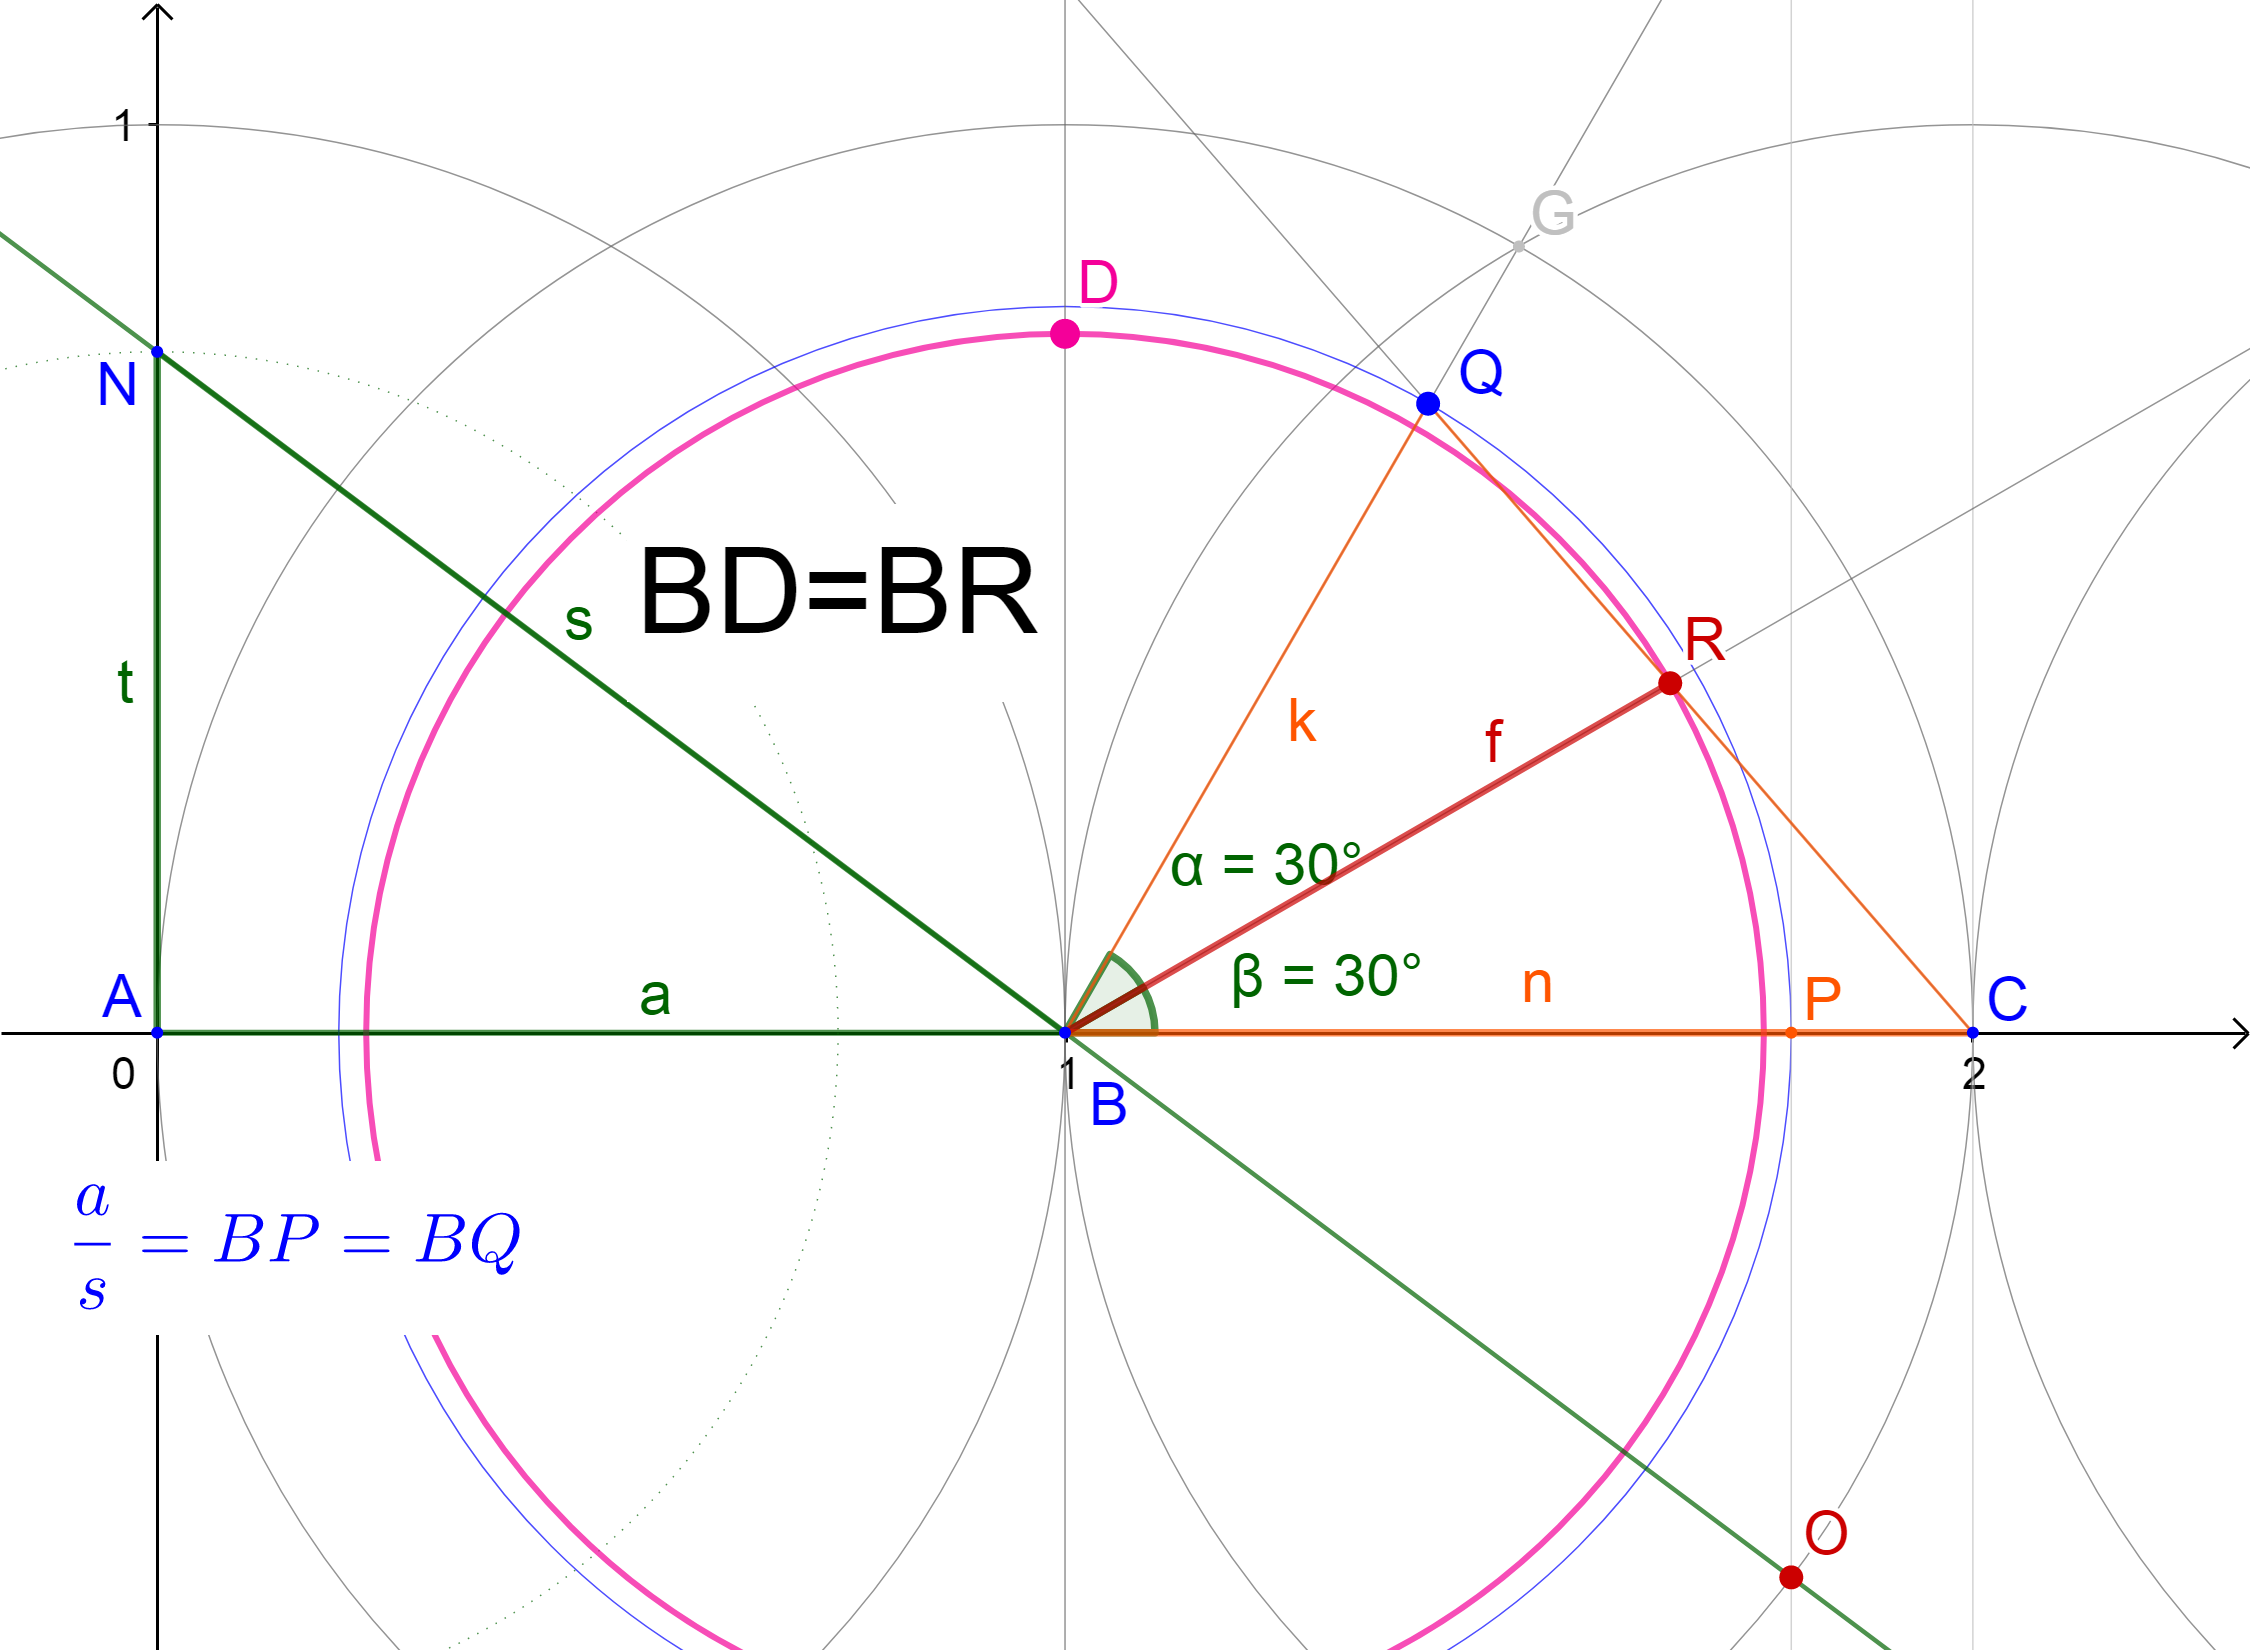
\includegraphics[scale=0.2]{img/bdBR.png}}
	\caption{Circle where radius = bisector BR}
	\label{circle}
\end{figure} 	
\newpage
	\item Now we have constructed a right triangle $\triangle BDC$ as shown in the fig. \ref{fig:bdc}. 
\begin{figure}[h]
	\centerline{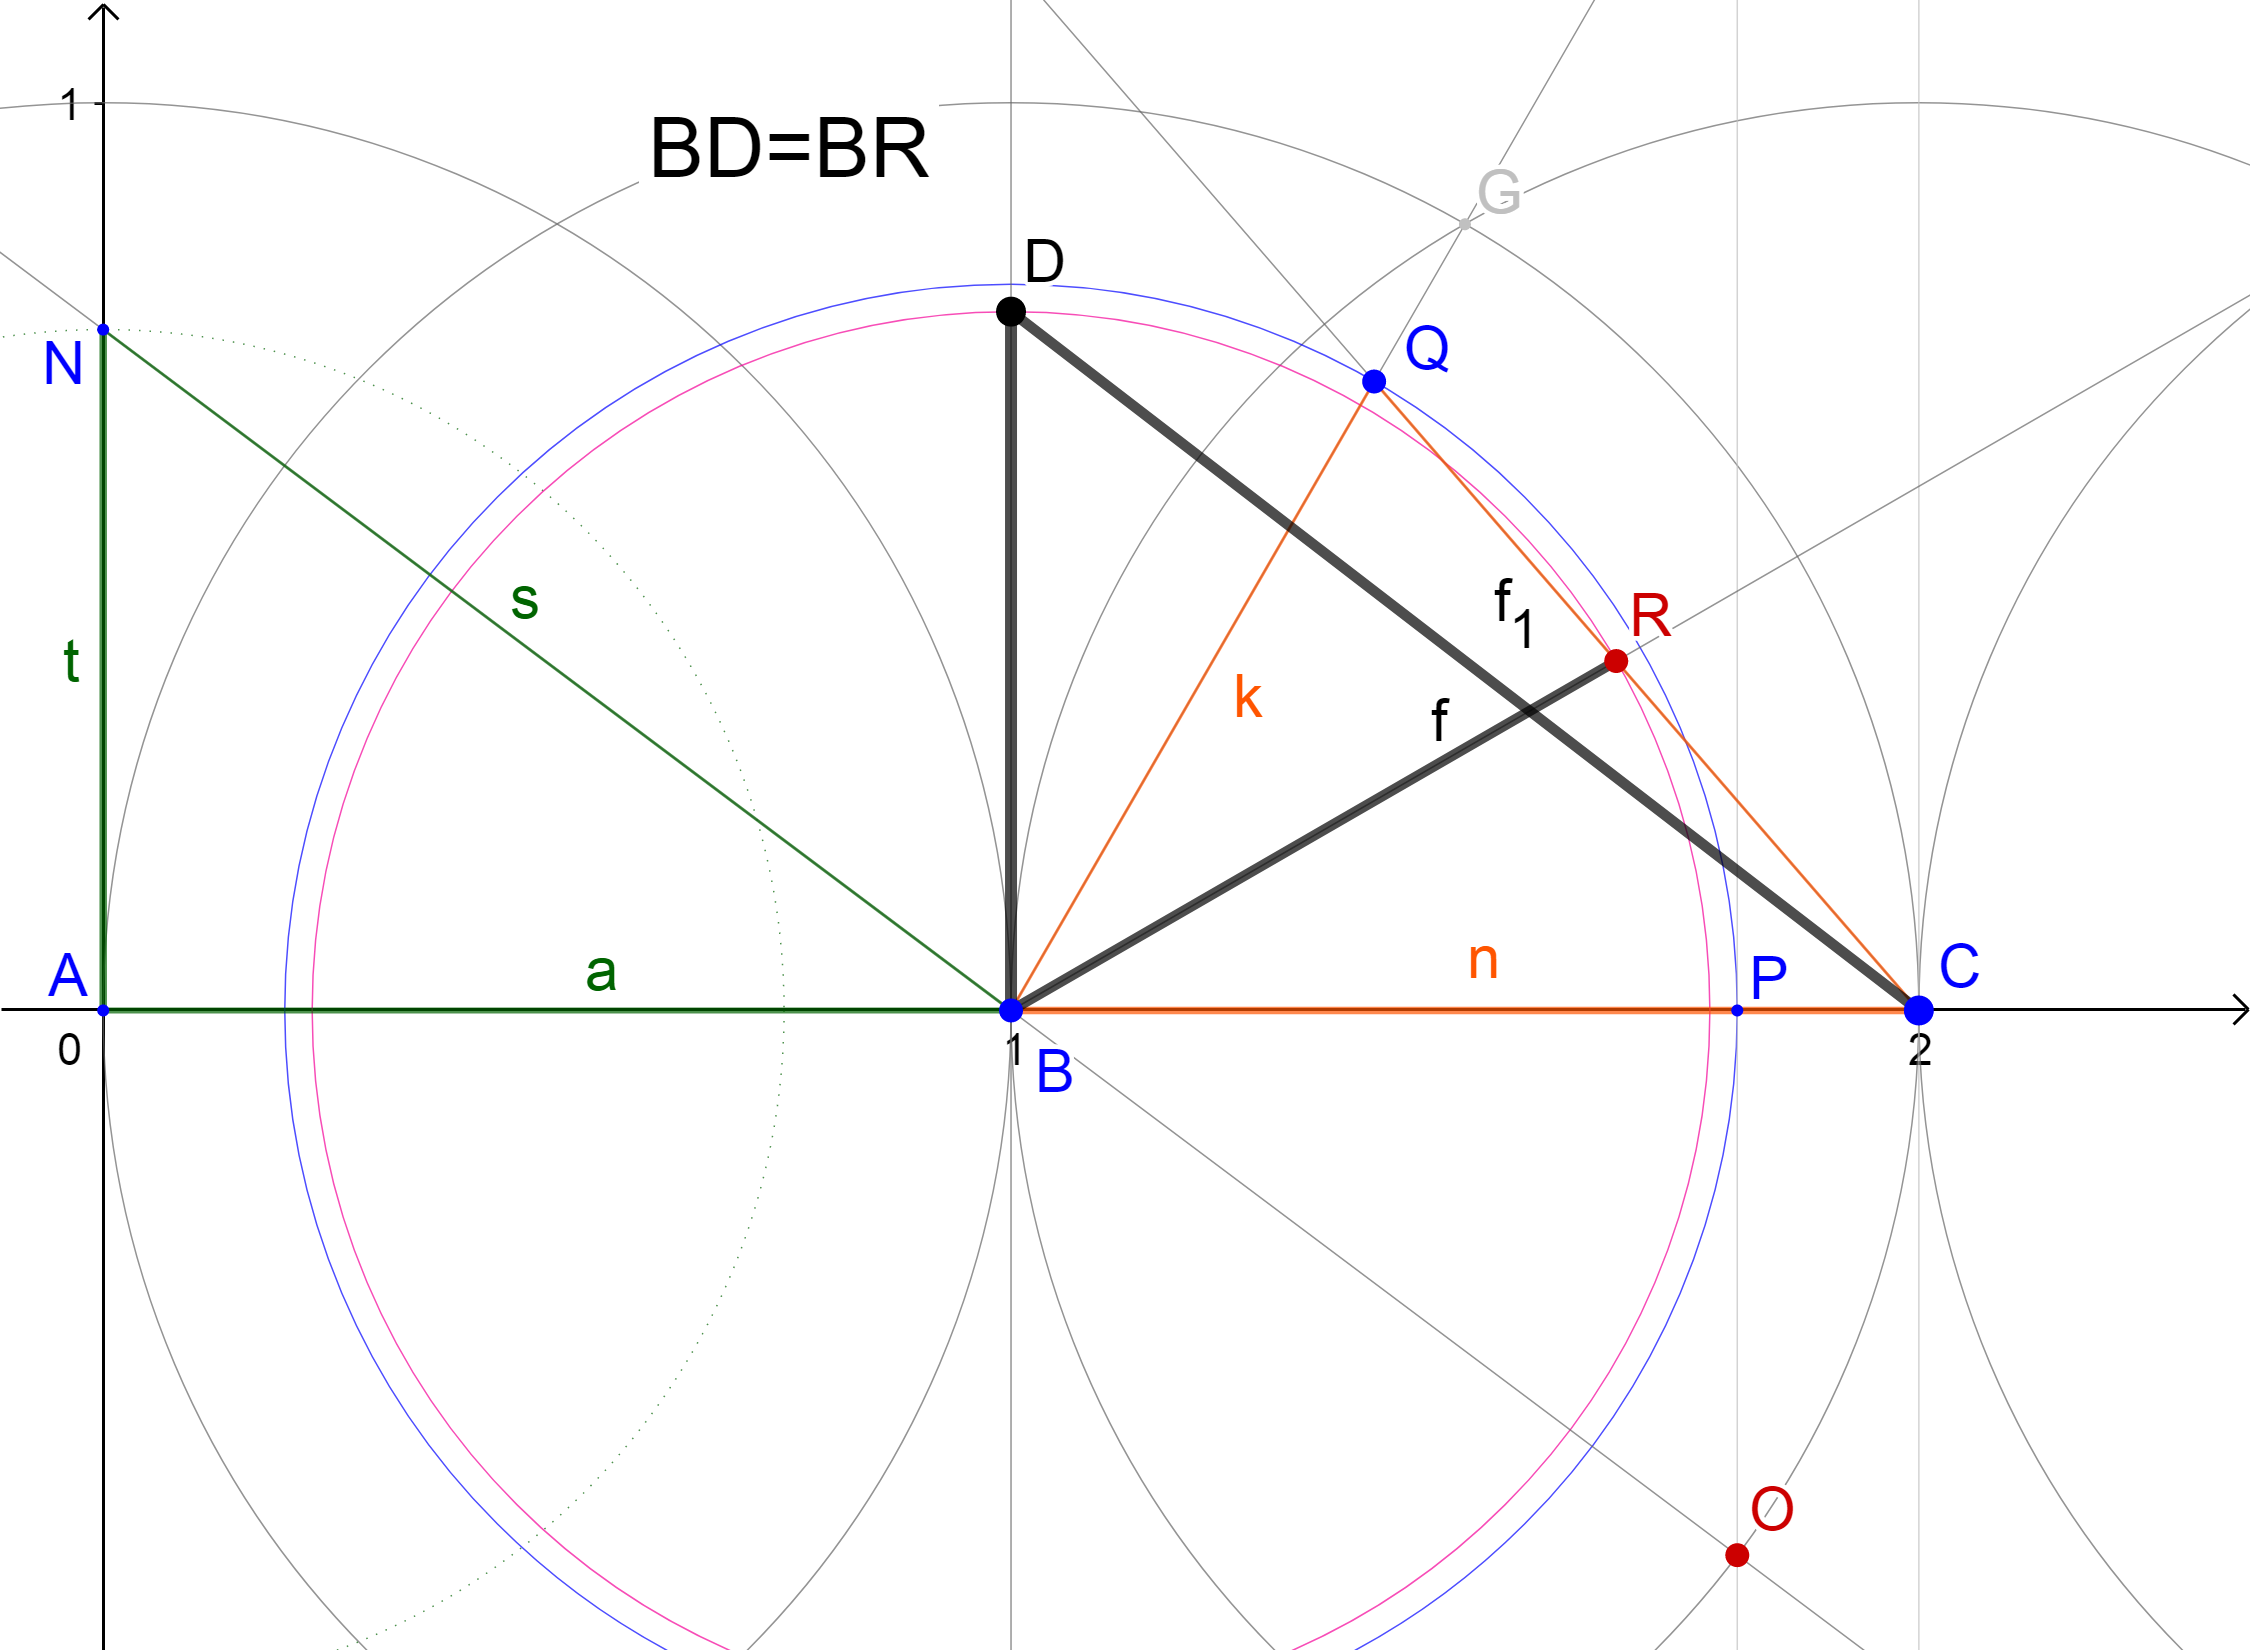
\includegraphics[scale=0.14]{img/BDC.png}}
	\caption{}
	\label{fig:bdc}
\end{figure}\\
So we have constructed the right triangle $\triangle BDC$.
\\
Now we need to repeat the following steps from the 3-rd step above:
\subitem calculate cosine value (step 3)
\subitem construct a circle (step 4)
\subitem construct a triangle with an angle of 60 degrees (step 5)
\subitem calculate the length of the bisector of the previously constructed triangle. (step 6)
\subitem construct the right triangle with shortest leg equal to the bisector from the previous step (step 7)
\subitem and repeat again from step 3
\subitem and so on...\\
\vspace{10mm}
\par
\textbf{\large {Conjecture:}}
\par

\textbf{Repeating these constructions, after the nth iteration, the hypotenuse ${DC}$ of $\triangle BDC$ tends to $\sqrt[3]{2}$ as the limit of recurrent sequence.}

\newpage
\section{Proof}
From the above constructions, we obtain a recurrent sequence:
\begin{equation}
( a_{1} > 0,  n \in \mathbb N ) \ \underset{n\to \infty }{lim} a_{n+1} = \dfrac{ 1 }{ \sqrt{ 1 + \left( \dfrac{ 2 a_{ n } }{ 1 + a_{ n } } \dfrac{ \sqrt{ 3 } }{ 2 } \right)^{2} } } =\dfrac{ 1 }{ \sqrt[3]{ 2 } }
\end{equation}\label{eq:recurr-relation}
Which follows from the following:
\begin{equation}
\sqrt[3]{2}= \underset{n\to \infty }{lim} \sqrt{1+b_{n}^2}
\end{equation}
\begin{equation}
b_{1}>0, \hspace{5pt} b_{n+1}=\dfrac{1}{\sqrt{1+b_{n}^{2}}},\ \hspace{5pt} b_{n+2}=\dfrac{2\times b_{n+1}}{1+b_{n+1}}\times\dfrac{\sqrt{3}}{2} ...
\end{equation}

Where $b_{n+1}$ is the cosine of the right triangle $\triangle CBD$ (see fig. \ref{fig:bdc}), \newline then $b_{n+2}=\dfrac{2\times b_{n+1}}{1+b_{n+1}}\times\dfrac{\sqrt{3}}{2}$ is the bisector $\overline{BR}$ of the triangle $\triangle BQC$ of the angle $\angle CBQ$ 60-degree, where the shortest leg $BQ$  is $ b_{n+1} $ 


\end{enumerate}
Let's expand and simplify this:
\[
a_{n+1} =\dfrac{ 1 }{ \sqrt{ 1 + \left( \dfrac{ 2 a_{ n } }{ 1 + a_{ n } }\dfrac{ \sqrt{ 3 } }{ 2 }\right)^{ 2 } } }
\]

\[
=\dfrac{1}{\sqrt{1+\dfrac{3a_{n}^{2}}{(a_{n}+1)^{2}}}}
\]

\[
=\dfrac{1}{\sqrt{ \dfrac{ 3 a_{ n }^{2}+( a_{ n }+1 )^{2} }{ ( a_{n}+1 )^{2} } } }
\]

\[ =\dfrac{1}{ \sqrt{ \dfrac{ 3a_{ n }^{ 2 }+( a_{ n }^2 + 2 a_{ n }+1 ) }{ ( a_{ n }+1 )^{ 2 } } } }
\]

\[
=\dfrac{ 1 }{\sqrt{\dfrac{4a_{n}^{2}+2a_{n}+1}{(a_{n}+1)^{2}}}}
\]

\[
=\dfrac{1}{\dfrac{ \sqrt{4a_{n}^{2}+2a_{n}+1} }{ \sqrt{(a_{n}+1)^{2}} } }
\]

\[
=\dfrac{ 1 }{ \dfrac{ \sqrt{ 4 a_{ n }^{ 2 } + 2 a_{ n } + 1 } }{ a_{ n } + 1 } }
\]

\[
=\dfrac{ | a_{n}+1 | }{ \sqrt{ 4 a_{ n }^{ 2 } + 2 a_{ n }+1} }
\]
Since ${ a_1 > 0 }$ we have that:
\[
a_{ n + 1 }=\dfrac{ a_{ n } + 1 }{ \sqrt{ 4 a_{ n }^{ 2 } + 2 a_{ n } + 1} }
\]
Now let's evaluate the limit of the sequence defined by: 
\begin{equation}\label{lim-def1}
(0 < a_{ 1 } < 1, n \in \mathbb N),
\underset{ n \to \infty }{lim} a_{ n+1 }=\dfrac{ a_{ n } + 1 }{ \sqrt{4 a_{ n }^{2} + 2 a_{n} + 1 } }
\end{equation}
\\
First we need to prove that $\{a_{n}\}$ is bounded. 
\\
Let $ a_{ 1 } = 1 $, $ a_{ n + 1 } = a_{k+1}$, $ k = n $ where $n \in \mathbb N$.
\\
We will prove by induction that $ a_{k + 1} < 1$.
\[
a_{k+1} =\dfrac{ a_{ 1 } + 1 }{ \sqrt{4 a_{ 1 }^{2} + 2 a_{1} + 1 } } \Rightarrow \dfrac{ 1 + 1 }{\sqrt{(4\times 1^{2})+(2\times 1)+1}}
\]

\[
= \dfrac{ 2 }{  \sqrt{ 7 } } = \dfrac{2}{2.645751} \approx 0.755929
\]

hence:
\[
a_{k+1} \approx 0.755929 < 1 
\]

Now we will prove that $ a_{ k + 2 } < 1 $
\[
a_{k + 2}=\dfrac{ a_{ k+1 } + 1 }{ \sqrt{ 4 a_{ k+1 }^{ 2 } + 2 a_{ k+1 } + 1} } \Rightarrow \dfrac{ 0.755929 + 1 }{  \sqrt{ (4\times 0.755929^{2} ) + ( 2\times 0.755929 ) + 1 } }
\]

\[
= \dfrac{ 1.755929 }{  \sqrt{4.797572}} = \dfrac{1.755929}{2.190336} \approx 0.801671 
\]

hence: \[ a_{k+2} \approx 0.801671 < 1 \]
So it is easy to see that $\{a_{k}\} < 1$ when $ a_{1} \le 1$.
\\
Therefore the sequence (1.8) is bounded above by $1$.
\\
Also ${\{a_{n}\}}$ is bounded below since $a_{1} > 0 $.

Since: 
\begin{equation}
f(x)=\dfrac{ x + 1 }{ \sqrt{ 4 x^{2} + 2 x + 1} }
\end{equation}
is a continuous function, we have that:
\begin{equation}
L=\underset{n\to \infty }{lim} a_{n+1}=\underset{n\to \infty }{lim}\dfrac{ a_{n}+1 }{ \sqrt{4a_{n}^{2}+2a_{n}+1} } = \dfrac{ L+1 }{ \sqrt{4L^{2}+2L+1} }
\end{equation}
\newpage
Therefore we need to solve the equation:
\\
\begin{equation}\label{l-eq}
L = \dfrac{ L + 1 }{ \sqrt{ 4 L^{ 2 } + 2 L + 1 } }
\end{equation}
\\
We need to multiply both sides by $\sqrt{4 L^2 + 2 L + 1}$ first:
\[ L + 1 = L \sqrt{4 L^2 + 2 L + 1}\] 

Isolate the radical to the left hand side:
\[L \sqrt{4 L^2 + 2 L + 1} = L + 1 \]

Raise both sides to the power of two:
\[L^2 (4 L^2 + 2 L + 1) = (L + 1)^2 \]

Expand out terms:
\[ 4 L^4 + 2 L^3 + L^2 = L^2 + 2 L + 1 \]

Subtract $L^2 + 2 L + 1$ from both sides:
\[ 4 L^4 + 2 L^3 - 2 L - 1 = 0 \]

The left hand side factors into a product with two terms:
\[ (2 L + 1) (2 L^3 - 1) = 0 \]

Split into two equations:
\[ 2 L + 1 = 0 \]

and
\[ 2 L^3 - 1 = 0 \]

Hence:
\[ 2 L = -1 \]

and
\[ 2 L^3 = 1 \]

Solve for L:
\[ L = -\dfrac{1}{2} \]

and:
\[ L^3 = \dfrac{1}{2} \]

since the $\{a_{n}\}>0$, the only possible choice is:
\[  L^3 = \dfrac{1}{2} \Rightarrow L = \frac{1}{\sqrt[3]{2}} \]
\newpage
\vspace{10mm}
Let's check the solution:
\[
\dfrac{ L + 1 } { \sqrt{ 4 L^2 + 2 L + 1} } \Rightarrow \dfrac{ 1 + \dfrac{ 1 }{ \sqrt[ 3 ]{ 2 } } } { \sqrt{ 4 \left( \dfrac{1}{ \sqrt[ 3 ]{ 2 } } \right)^2 + \dfrac{2}{\sqrt[ 3 ]{ 2 } } + 1 } }
\]

\[
= \dfrac{ 2 + 2^{ 2/3 } }{ 2 + 2\sqrt[ 3 ]{ 2 } }
\]

\[
= \dfrac{ 2 + \sqrt[3]{ 4 } }{ 2 + 2\sqrt[ 3 ]{ 2 } } = 0.793700525984
\]
\vspace{5mm}
Hence:
\[
L = 0.793700525984
\]
\vspace{5mm}
While $ \dfrac{1}{\sqrt[ 3 ]{ 2 } } = 0.793700525984... $ rounded to 12 decimal places.

\vspace{10mm}
So this proves that $a_{n} \to \dfrac{1}{\sqrt[3]{2}}$ as $n\to \infty$  in the recurrence relation:
\[
( a_{1} > 0,  n \in \mathbb N ) \ \underset{n\to \infty }{lim} a_{n+1} = \dfrac{ 1 }{ \sqrt{ 1 + \left( \dfrac{ 2 a_{ n } }{ 1 + a_{ n } } \dfrac{ \sqrt{ 3 } }{ 2 } \right)^{2} } } =\dfrac{ 1 }{ \sqrt[3]{ 2 } }
\]
 \newpage
 \par
We have proved that the recurrent sequence $1.5$ is equal to $\sqrt[3] {2}$.
\newline
\par
Notice that the physical world is limited in its minimum values by the Planck length:

\[ l_{p} = 1,616255(18) \times 10^{-35} \]

which means that all values less than the Planck length have no physical meaning. In order to reach the maximum possible value limited by the Planck length we need to perform the above constructions 57 times.
\\
\par
Indeed we find a way to construct $\sqrt[3]{2}$ using only a compass and straightedge. 
\\
\par 
Most importantly, we discovered a new fundamental property of an equilateral triangle that is directly related to the cube root of two.
\\

\begin{figure}[h]
	\centering
	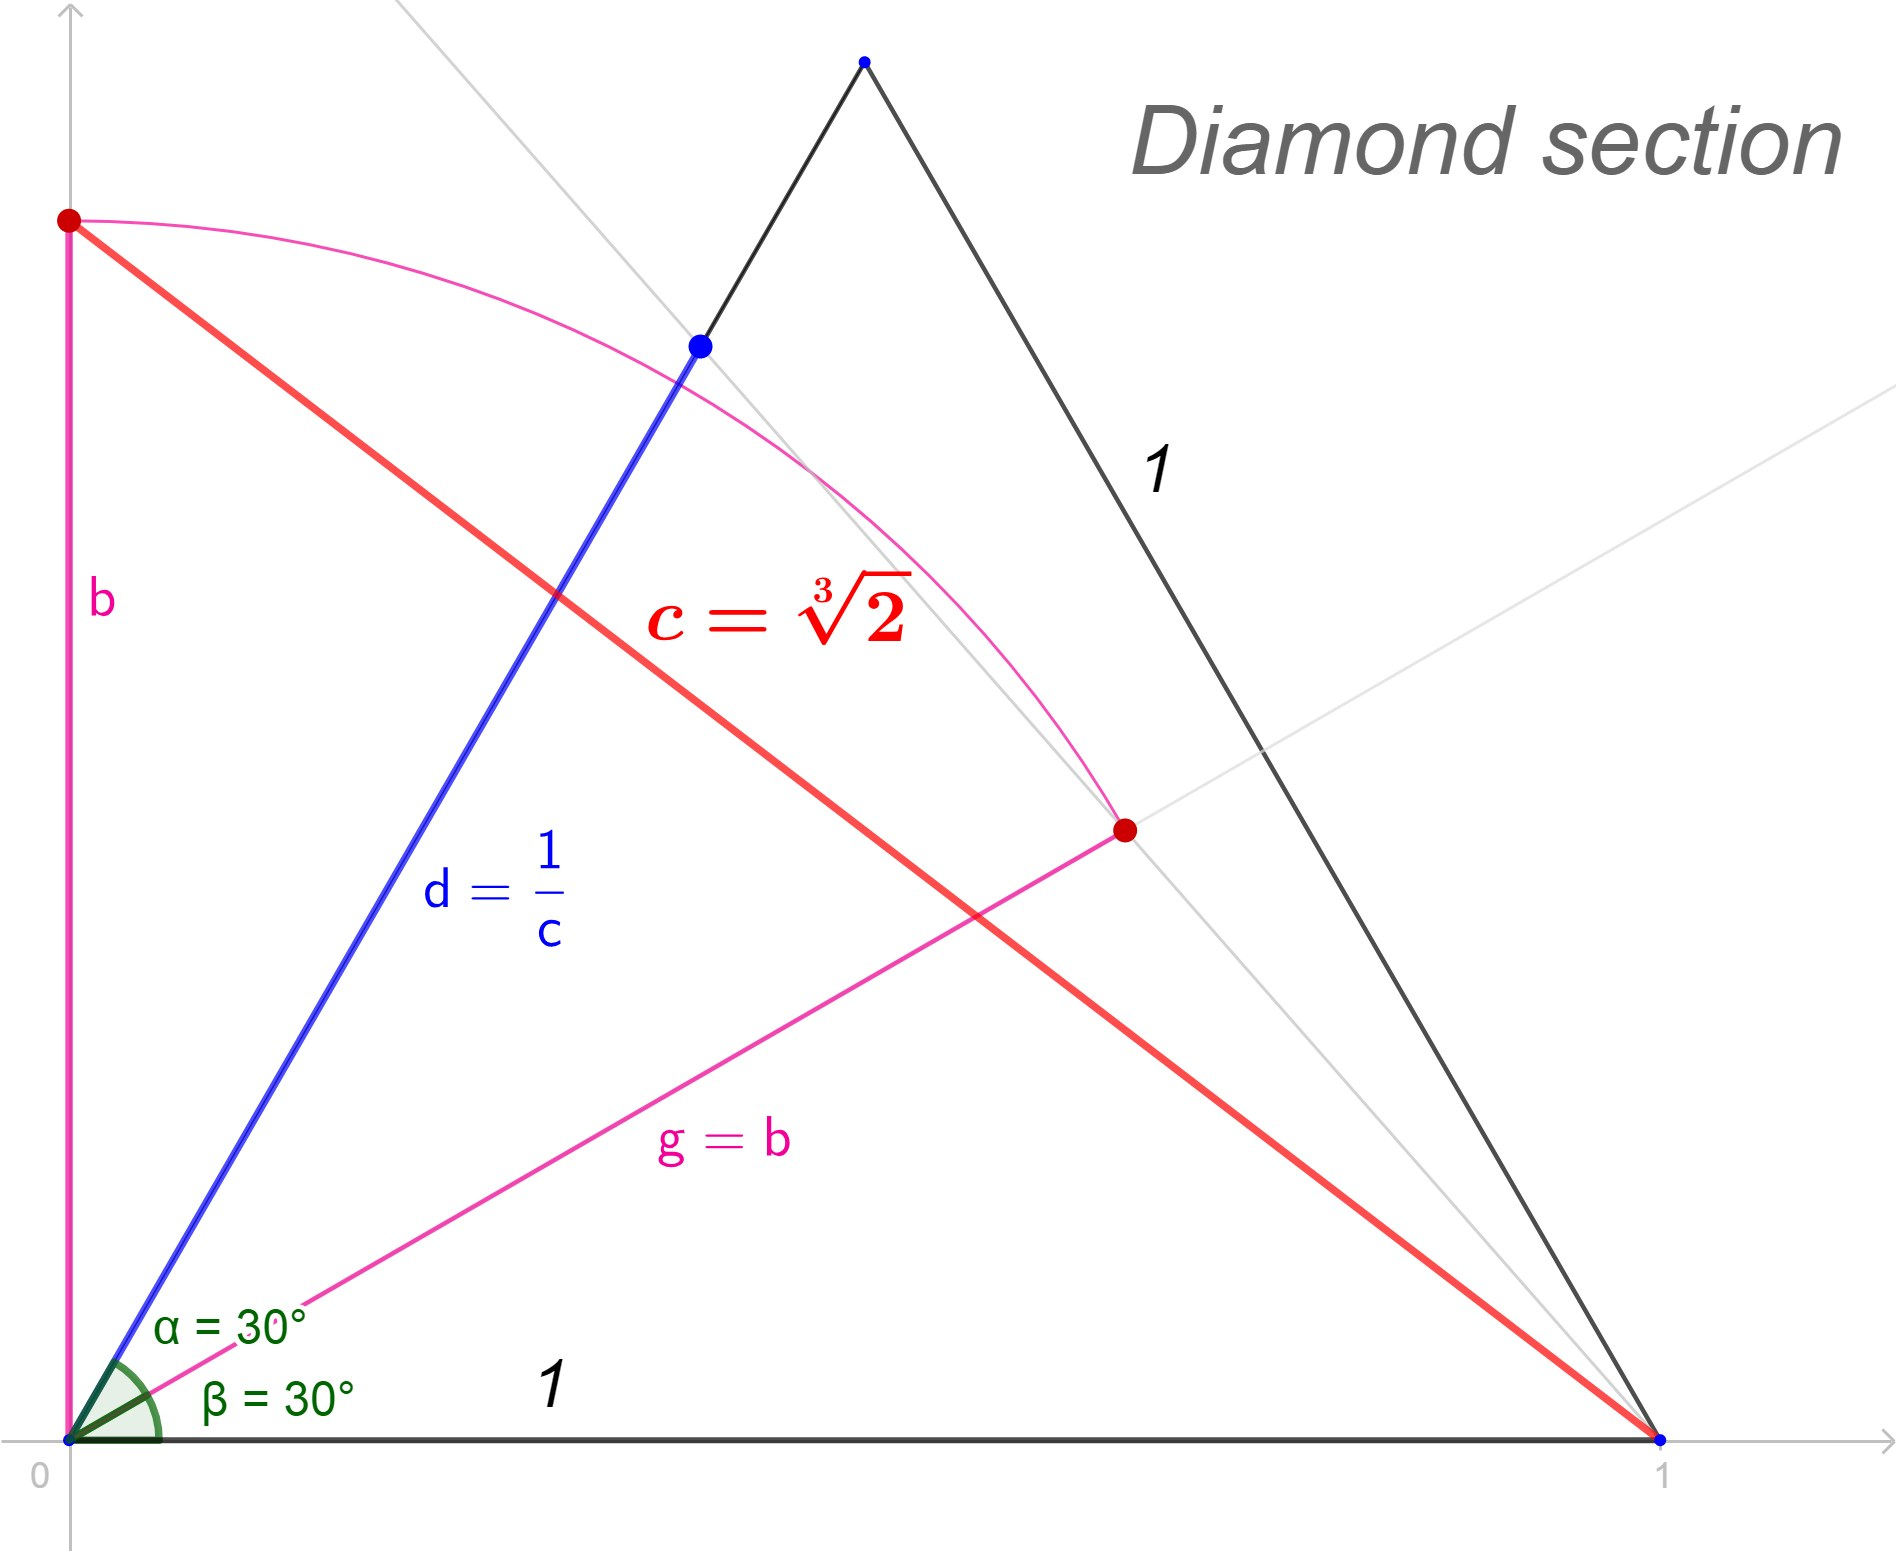
\includegraphics[width=0.7\linewidth]{images/ds_def.jpg}
	
	\label{fig:Diamond Section}
\end{figure}

\newpage

\section{Appendix}
\textbf{\large The square root of the golden ratio}

\begin{figure}[h]
	\centering
	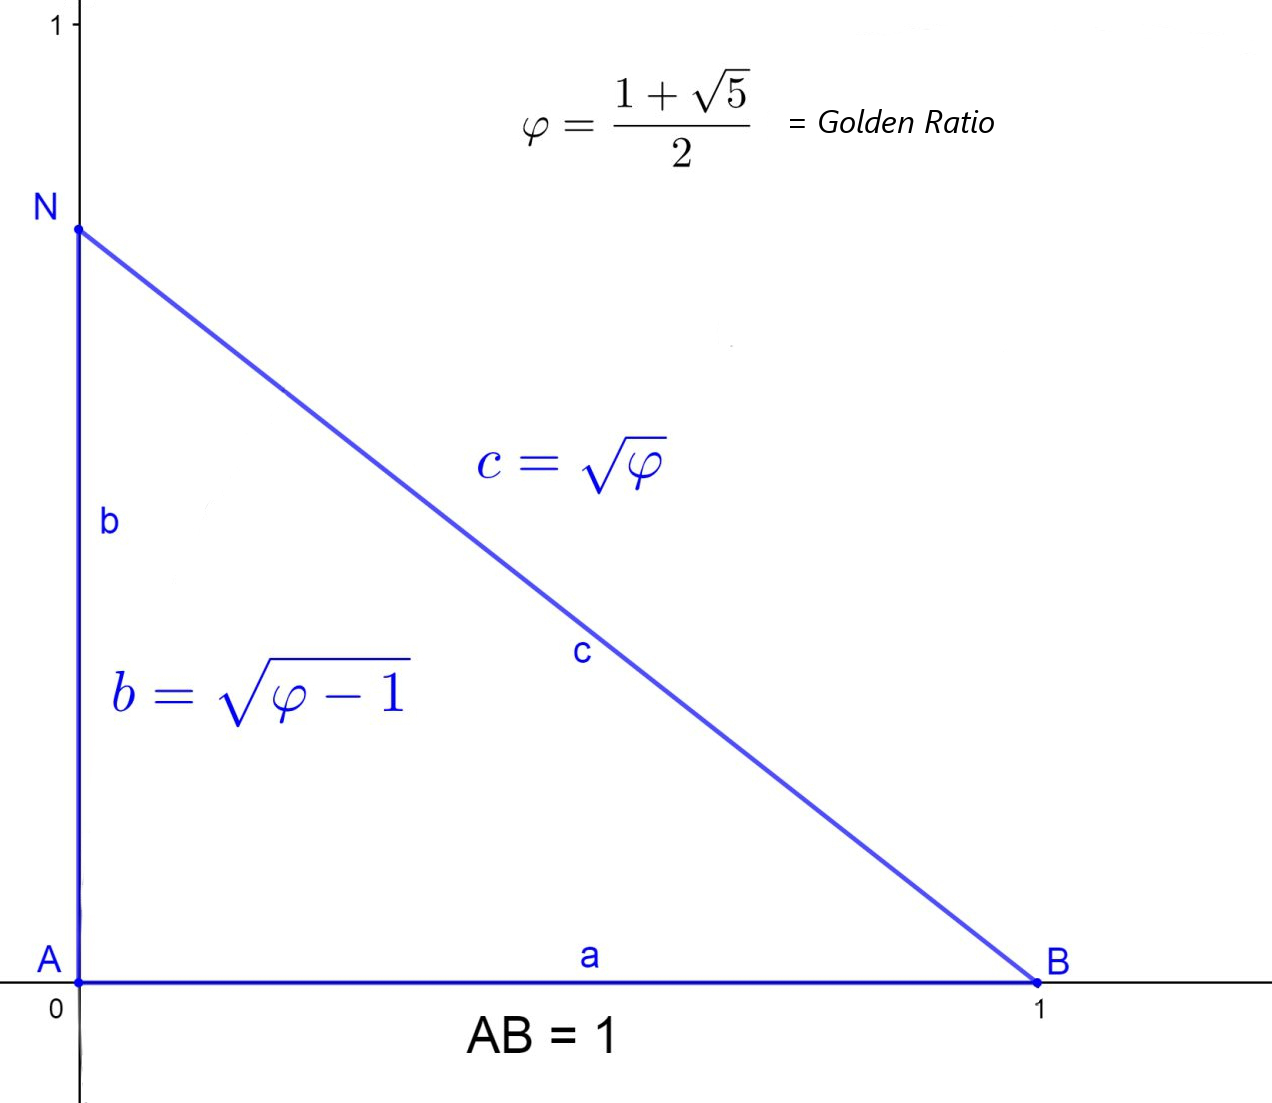
\includegraphics[width=0.7\linewidth]{images/phi-triangle.jpg}
	\caption{Right triangle}
	\label{fig:phi-triangle}
\end{figure}
\par Let's take an \textbf{arbitrary} shortest leg $b$ of the right triangle \ref{fig:phi-triangle} with a long leg $a=1$ and recursively do the following: find the hypotenuse using the formula {c }=$\sqrt{a^2+b^2}$, then get $ b_{1 }$ as the reciprocal of the hypotenuse $c$
\begin{equation}
\dfrac{1}{\sqrt{a^2+b^2}} = \dfrac{1}{c} = b_{1}; \   
\end{equation} 
Now let's take $b_{1}$ as a small leg of a right triangle, where $a=1$, and repeat the above steps according to the formula:
\begin{equation}
\lim_{n\to\infty}\ \ \ \dfrac{1}{\sqrt{a^2+b^2}} = b_{1}; \   \dfrac{1}{\sqrt{a^2+b_{1}^2}} = b_{2}; \   \dfrac{1}{\sqrt{a^2+b_{2}^2}}=b_{3}; \ ... \dfrac{1}{\sqrt{a^2+b_{n-1}^2}}=b_{n}\ \label{eq:1}
\end{equation} 
After the n-th number of iterations, we will get the following values:
\begin{equation}
a=1; \ \ \ \ 
\\
b=\sqrt{\varphi-1}; \ \ \ \ 
\\
c=\sqrt{\varphi};
\end{equation}
\\
Thus, the value of a small leg $b$ in the limit of the recursive sequence \ref{eq:1} tends to $\sqrt{\varphi-1}$, and the hypotenuse ${c}$ tends to $\sqrt{ \varphi}$, where $\varphi $ = Golden ratio = $1.6180339887...$ (see fig. \ref{fig:phi-triangle})
\\
 
\newpage


\begin{minipage}{0.8\textwidth}

\title{text}

	
\section{Links}

\large Author:

e-mail: \textbf{jobspace@yandex.com} \\
github: \url{https://github.com/AlmasAskarbekov}

\section{Thanks}
\url{https://geogebra.org}
\\

\end{minipage}
\vspace{365pt}
\hrule
\ 
\\
\emph{Keywords: Doubling the cube, the Delian problem, Geometric problems of Antiquity, geometry, ancient mission impossible of geometry}




\begin{thebibliography}{5}
\bibitem{A}
\url{https://en.wikipedia.org/wiki/Doubling_the_cube}
\bibitem{B}
\url{https://oeis.org/A002580}
\end{thebibliography}

\vspace{465pt}

%%%%%%Dedicated to Delos%%%%%%%% 
\end{document}